\documentclass[a4paper]{article}
\usepackage[utf8]{inputenc}
\usepackage[spanish, es-tabla, es-noshorthands]{babel}
\usepackage[table,xcdraw]{xcolor}
\usepackage[a4paper, footnotesep = 1cm, width=20cm, top=2.5cm, height=25cm, textwidth=18cm, textheight=25cm]{geometry}
%\geometry{showframe}

\usepackage{tikz}
\usepackage{amsmath}
\usepackage{amsfonts}
\usepackage{amssymb}
\usepackage{float}
\usepackage{graphicx}
\usepackage{caption}
\usepackage{subcaption}
\usepackage{multicol}
\usepackage{multirow}
\setlength{\doublerulesep}{\arrayrulewidth}
\usepackage{booktabs}

\usepackage{hyperref}
\hypersetup{
    colorlinks=true,
    linkcolor=blue,
    filecolor=magenta,      
    urlcolor=blue,
    citecolor=blue,    
}

\newcommand{\quotes}[1]{``#1''}
\usepackage{array}
\newcolumntype{C}[1]{>{\centering\let\newline\\\arraybackslash\hspace{0pt}}m{#1}}
\usepackage[american]{circuitikz}
\usetikzlibrary{calc}
\usepackage{fancyhdr}
\usepackage{units} 

\graphicspath{{../Ejercicio-1/}{../Ejercicio-2/}{../Ejercicio-3/}{../Ejercicio-4/}}

\pagestyle{fancy}
\fancyhf{}
\lhead{22.01 Teoría de Circuitos}
\rhead{Mechoulam, Lambertucci, Rodriguez Turco, Londero, Galdeman}
\rfoot{\centering \thepage}

\newcommand\underrel[2]{\mathrel{\mathop{#2}\limits_{#1}}}

\usepackage{circuitikz}
\usepackage{xcolor}
\usepackage{amsmath}

\begin{document}


\section{Comportamiento de Amplificadores Operacionales.}

\subsection{Introducción y modelos.}
En el presente punto se analizan las limitaciones del amplificador operacional \textbf{LM324} en las configuraciones inversora y no inversora.

Un amplificador operacional es un dispositivo electrónico el cual, dependiendo de la tensión de entrada, fija una tensión de salida. Estos se pueden modelar de la siguiente forma:
\begin{figure}[H]	
	\centering
	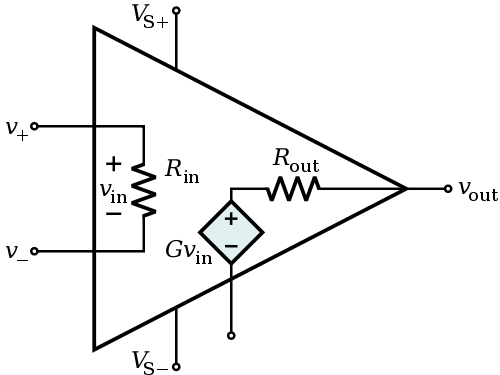
\includegraphics[width=0.7\textwidth]{Ejercicio1/Imagenes/Basicopamp.png}
	\caption{Modelo básico del amplificador operacional.}
	\label{fig:Basicopamp}
\end{figure}
donde típicamente $R_{in}\approx \infty$ y $R_{out} \approx 0$

\subsubsection{Modelo ideal.}
En el modelo ideal realimentado por el borne inversor ($V^-$), las hipótesis con las que se trabaja son:
\begin{align} V^+ = V^- \end{align}
\begin{align}V_{Out} \underrel{A_{Vol}\to \infty}{=} A_{Vol} \cdot (V^+ - V^-) \end{align}
\begin{align} R_{in}=\infty   \thinspace;\thinspace R_{Out} = 0 \end{align}


\subsubsection{Modelo $A_{Vol}$ finito.}
Para este modelo se le agregan idealidades al modelo anterior.
\begin{align}V_{Out} = A_{Vol} \cdot (V^+ - V^-)
\label{eq:vout}
\end{align}

Si bien la realimentación negativa intentará hacer que la diferencia entre $V^+$ y $V^-$ sea 0, no es algo que se asume en este modelo.

\subsubsection{Modelo polo dominante.}
Este modelo es el más cercano al real que se trata en el presente trabajo. Los amplificadores operacionales poseen un polo dominante, el cual está diseñado intencionalmente por el fabricante, para cubrir algunos problemas que surgen al trabajar con mayores frecuencias. Estos dispositivos cuentan con una serie de polos debido a capacidades parásitas propias de la construcción. El polo dominante es introducido para evitar que estos polos desestabilicen el circuito al introducir una inversión en el lazo de realimentación, a altas frecuencias.

\begin{figure}[H]	
	\centering
	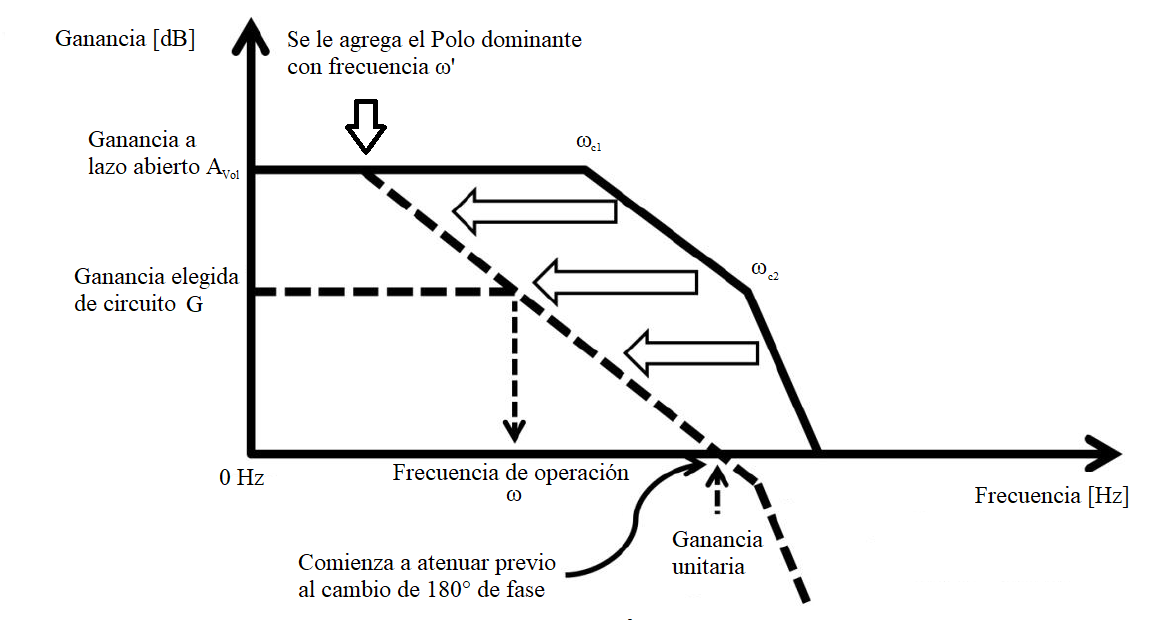
\includegraphics[width=\textwidth]{Ejercicio1/Imagenes/dompole.png}
	\caption{Modelo polo dominante.}
	\label{fig:dompole}
\end{figure}

También se define un ``Ancho de Banda'', con el cual se puede trabajar; comúnmente el dato con el que se trabaja es el conocido como GBP (Gain Bandwidth Product), el cual sigue la siguiente relación:

\begin{align} GBP= A_{Vol} \cdot \omega' \end{align}
donde $\omega'$ es la frecuencia del polo dominante a lazo abierto. También se cumple que 

\begin{align} GBP=\omega \cdot G \end{align}
donde $\omega$ es la frecuencia de corte del circuito en el que esté aplicado y G la ganancia del mismo.
Finalmente la ecuación principal que rige este modelo es (\ref{eq:vout}) con la singularidad de que:
\begin{equation}
	A_{Vol} = A_{Vol}(s) = \frac{A_{vol}}{1+\frac{s}{\omega '}}
	\label{eq:PoloDom}
\end{equation}  

\subsection{Configuración inversora y no inversora.}
La cátedra propone dos modelos de circuitos diferentes para analizar. Estos son los presentados a continuación:

\begin{figure}[H]
\begin{center}
\begin{circuitikz}
	\node [op amp](A1){};
	\draw (A1.-) to[short] ++(-2.5,0) to[R, l_= $R_1$] ++(-1.5,0) to[short, -o] node[ocirc,label=left:$V_{in}$]{} ++(-1,0);
	\draw (A1.-) to[open] ++(-2,0) to[R, l_= $R_3$] ++(0,-2) node[ground]{};
	\draw (A1.-) node[label=south:$V^-$]{};
	\draw (A1.+) node[label=south:$V^+$]{};
	\draw (A1.+) to[short] ++(-1,0) to[short] ++(0,-1) node[ground]{};
	\draw (A1.-) to[short] ++(0,1.5) to[R, l = $R_2$] ++(3,0) to[short] ++(0,-2) to[R, l = $R_4$] ++(0,-1.5) node[ground]{};
	\draw (A1.out) to[short, -o] ++(1,0) node[ocirc,label=right:$V_{out}$]{};
	\end{circuitikz}
	\caption{Configuración inversora.}
	\label{fig:ConfInv}
\end{center}
\end{figure}

\begin{figure}[H]
\begin{center}
\begin{circuitikz}
	\node [op amp](A1){};
	\draw (A1.-) to[short] ++(-1.5,0) to[R, l_=$R_1$] ++(-1.5,0) to[short] ++(-1,0) node[ground]{};
	\draw (A1.-) node[label=south:$V^-$]{};
	\draw (A1.+) node[label=south:$V^+$]{};
	\draw (A1.-) to[short] ++(0,1.5) to[R, l = $R_2$] ++(3,0) to[short] ++(0,-2);
	\draw (A1.+) to[short] ++(-1,0) to[R, l = $R_4$] ++(0,-1.5) node[ground]{};
	\draw (A1.out) to[short, -o] ++(1,0) node[ocirc,label=right:$V_{out}$]{};
	\draw (A1.+) to[short] ++(-1,0) to[R, l= $R_3$] ++(-2,0) to[short, -o] node[ocirc,label=left:$V_{in}$]{} ++(-1,0);
	\end{circuitikz}
	\caption{Configuración no inversora.}
	\label{fig:ConfNoInv}
\end{center}
\end{figure}

Para ambos, y debido a que se utiliza el mismo operacional en cada caso, se obtuvieron los siguientes datos de la hoja de datos del fabricante:
\begin{table}[H]
\begin{center}
\begin{tabular}{|c|c|c|c|c|}
\hline
%\multicolumn{5}{|c|}{}                                      \\ \hline
\textbf{$A_{vol}$} & $Max \ V_{in}$ & $V_{cm}$ & Slew rate             & GBW \\ \hline
100 k              & $32 \ V$         & $VCC \ - \ 1.5 \ V$  & 0.3 $\frac{V}{\mu s}$ & $1 \ MHz$  \\ \hline
\end{tabular}
\caption{Datos pertinentes al operacional.}
\label{tab:datos}
\end{center}
\end{table}

%%%%%%%%%%%%%%%%%%%%%%%%%%%%
\subsubsection{Calculo Analítico del Circuito Inversor.}
Lo primero que se realizó fue utilizar el equivalente de Thevenin para simplificar los cálculos analíticos.

\begin{figure}[H]
\begin{center}
\begin{circuitikz}
	\node [op amp](A1){};
	\draw (A1.-) to[short] ++(-1,0) to[R, l = $R_{Thevenin}$] ++(-2,0) to[short, -o] node[ocirc,label=left:$V_{Thevenin}$]{} ++(-0.5,0);
	\draw (A1.-) node[label=south:$V^-$]{};
	\draw (A1.+) node[label=south:$V^+$]{};
	\draw (A1.+) to[short] ++(-1,0) to[short] ++(0,-1) node[ground]{};
	\draw (A1.-) to[short] ++(0,1.5) to[R, l = $R_2$] ++(3,0) to[short] ++(0,-2) to[R, l = $R_4$] ++(0,-1.5) node[ground]{};
	\draw (A1.out) to[short, -o] ++(2,0) node[ocirc,label=right:$V_{out}$]{};
	\end{circuitikz}
	\caption{Equivalente de Thevenin del circuito inversor.}
	\label{fig:Thevenin}
\end{center}
\end{figure}

Teniendo en cuenta que 
\begin{align}
	V_{Thevenin} = V_{in} \cdot \frac{R_3}{R_1+R_3} \\
	R_{Thevenin} = \frac{R_1\cdot R_3}{R_1+R_3}
\label{eq:thev}
\end{align} 

Se considera primero caso genérico y una vez terminado el desarrollo, se toman las aproximaciones necesarias para los diversos casos pedidos.
\begin{align}
V_{Out}= A_{Vol}(\omega) \cdot (V^+ - V^-)
\label{equ:avoligualvo}
\end{align}
\begin{align}
V^+=0\end{align}
\begin{align}\frac{V_{Th}-V^-}{R_{Th}}=\frac{V^--V_{Out}}{R_2}
\label{eq:nodeInv}
\end{align}

Despejando para $V_{Out}$ se llega a que:
\begin{align}
\label{eq:Vout}
V_{Out}=-V_{in} \cdot \frac{R_3}{R_1+R_3} \cdot \frac{\frac{R_2}{R_{Th}+R_2}\cdot A(\omega)}{1+\frac{R_{Th}}{R_{Th}+R_2}\cdot A(\omega)}
\end{align}
sabiendo que la transferencia es $ H(s)=\frac{V_{Out}}{V_{in}} $.

Para el caso de $A_{Vol}=\infty$ simplemente basta tomar:
\begin{align}\lim_{A_{Vol}\to\infty} - \frac{R_3}{R_1+R_3} \cdot \frac{\frac{R_2}{R_{Th}+R_2}\cdot A(\omega)}{1+\frac{R_{Th}}{R_{Th}+R_2}\cdot A(\omega)} = -\frac{R_3}{R_1+R_3}\cdot\frac{R_2}{R_{Th}}=-\frac{R_2}{R_1}\end{align}

Para el caso de $A_{Vol}$ finito solamente se reescribirá (\ref{eq:Vout}).

\begin{align}
H(s)= -\frac{R_2\cdot A_{Vol}}{R_1\cdot R_3+R_1\cdot R_3 \cdot A_{Vol} +R_2\cdot R_3+R_2\cdot R_1}
\label{eq:AvolFinite}
\end{align}

Finalmente el caso el cual incluye el polo dominante alcanza con tomar lo especificado en (\ref{eq:PoloDom}), donde $\omega'$ es la frecuencia del polo dominante. Utilizando (\ref{eq:PoloDom}) y (\ref{eq:AvolFinite}) se llega a la expresión:
\begin{align}
\label{eq:polodom}
H(s)=-\frac{A_0R_2R_3}{A_0R_1R_3+R_1R_2+R_1R_3+R_2R_3} \cdot \left[1+s \left( \omega' \cdot \frac{A_0R_1R_3+R_1R_2+R_1R_3+R_2R_3}{R_1R_2+R_1R_3+R_2R_3} \right)^{-1} \right]^{-1}
\end{align}

De (\ref{eq:polodom}) se obtiene la frecuencia de corte del sistema.
\begin{align}
f_c=\frac{\omega'}{2\pi} \cdot \frac{A_0R_1R_3+R_1R_2+R_1R_3+R_2R_3}{R_1R_2+R_1R_3+R_2R_3}
\end{align}
Luego, teniendo en cuenta que
\begin{align}
\omega'=\frac{GBW}{A_0} = 2 \pi\cdot 10 \ Hz \approx 62.83 \ Hz
\end{align}

Para este grupo, los valores de resistencias asignados se presentan a continuación:
\begin{table}[H]
\begin{center}
\begin{tabular}{|c|c|c|c|}
\hline
\textbf{Caso:}              & \textbf{1}               & \textbf{2}               & \textbf{3}                \\ \hline
$R_1=R_3$                   & $7.5$                      & $7.5$                      & $75$                       \\ \hline
$R_2$                       & $75$                       & $7.5$                      & $7.5$                       \\ \hline
\multicolumn{1}{|c|}{$R_4$} & \multicolumn{1}{l|}{$30$} & \multicolumn{1}{l|}{$30$} & \multicolumn{1}{l|}{$300$} \\ \hline
\end{tabular}
\caption{Valores de resistencias en $k\Omega$.}
\label{tabla:resasignadas}
\end{center}
\end{table}

Para estos casos se calculó la ganancia considerando $A_{Vol}$ finito e infinito. Además, se calculó la frecuencia de corte del sistema para $A(\omega)$.

\begin{table}[H]
\begin{center}
\begin{tabular}{|c|c|c|c|}
\hline
\textbf{Caso}            & \textbf{1} & \textbf{2} & \textbf{3} \\ \hline
\textbf{$H(s)_{\infty}$} & 10         & 1          & 0.1        \\ \hline
\textbf{$H(s)_{Finito}$} & 9.9998     & 0.9999     & 0.0999     \\ \hline
\textbf{$f_c$}           & 47.62 kHz   & 333.34 kHz  & 833.34 kHz     \\ \hline
\end{tabular}
\caption{Ganancias y frecuencias de corte de los circuitos inversores.}
\label{tabla:gananciasinv}
\end{center}
\end{table}

Luego se procedió a realizar los gráficos de $H(s)$ cpn las distintas consideraciones de $A_{Vol}$ para cada uno de los 3 casos.
\begin{figure}[H]	
	\centering
	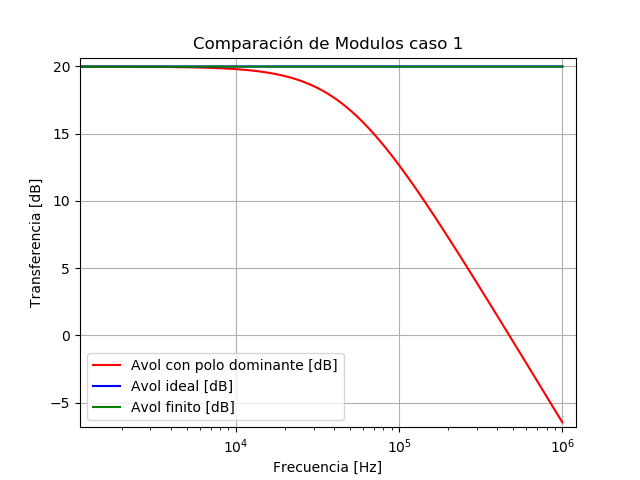
\includegraphics[width=\textwidth]{Ejercicio1/Imagenes/HCompC1.png}
	\caption{$A_{Vol}(\omega)$ Caso 1.}
	\label{fig:AvolC1}
\end{figure}
\begin{figure}[H]	
	\centering
	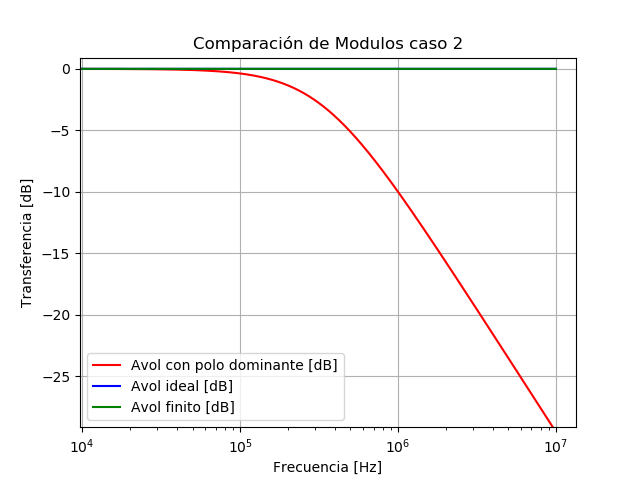
\includegraphics[width=\textwidth]{Ejercicio1/Imagenes/HCompC2.png}
	\caption{$A_{Vol}(\omega)$ Caso 2.}
	\label{fig:AvolC2}
\end{figure}
\begin{figure}[H]	
	\centering
	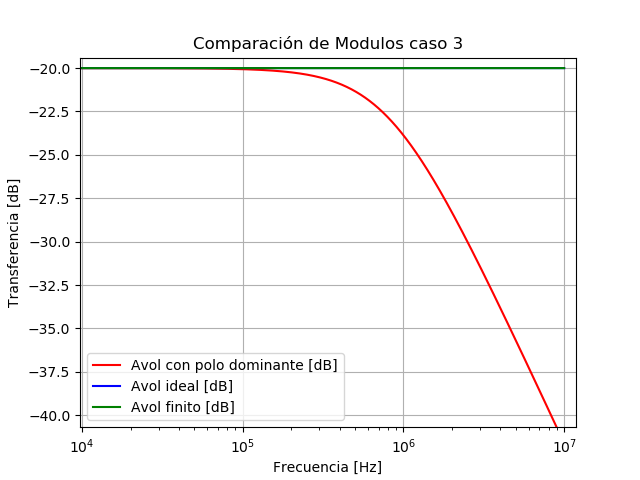
\includegraphics[width=\textwidth]{Ejercicio1/Imagenes/HCompC3.png}
	\caption{$A_{Vol}(\omega)$ Caso 3.}
	\label{fig:AvolC3}
\end{figure}

Se puede apreciar que cuanto más baja sea la ganancia, mayor será el ancho de banda, y que a partir de la frecuencia de corte cada sistema el opamp comienza a atenuar.

El error de utilizar el caso de $A_{Vol}$ ideal en lugar del caso con polo dominante se calculó como:
\begin{equation}
	Error = \frac{|A_{Vol}(\omega)-A_{Vol-Ideal}|}{A_{Vol}(\omega)}
	\label{equ:error}
\end{equation}

obteniendo los siguientes gráficos:

\begin{figure}[H]	
	\centering
	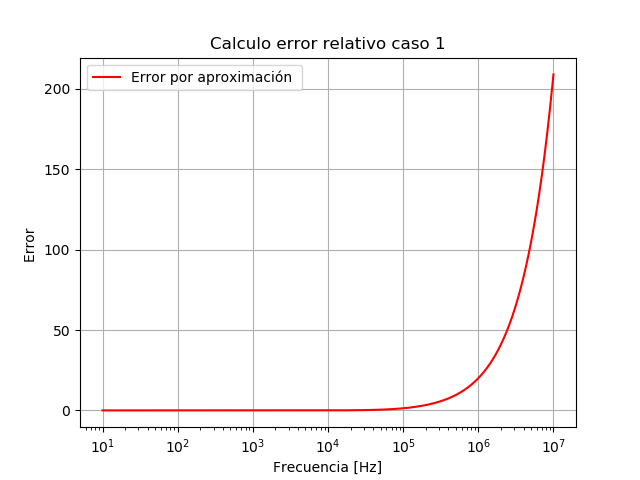
\includegraphics[width=\textwidth]{Ejercicio1/Imagenes/error1.png}
	\caption{Error relativo por aproximar Caso 1.}
	\label{fig:e1}
\end{figure}
\begin{figure}[H]	
	\centering
	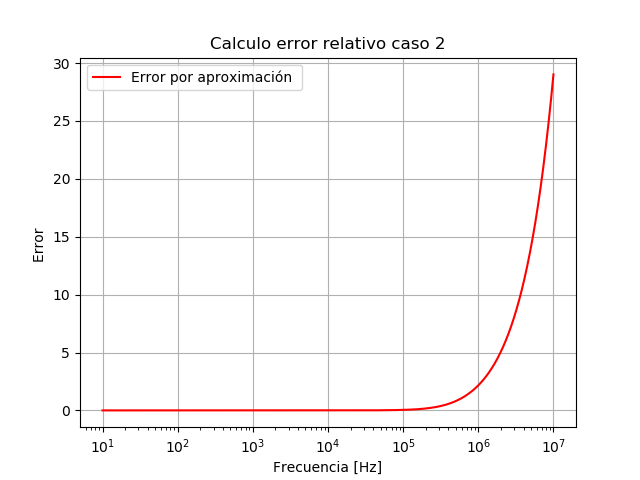
\includegraphics[width=\textwidth]{Ejercicio1/Imagenes/error2.png}
	\caption{Error relativo por aproximar Caso 2.}
	\label{fig:e2}
\end{figure}
\begin{figure}[H]	
	\centering
	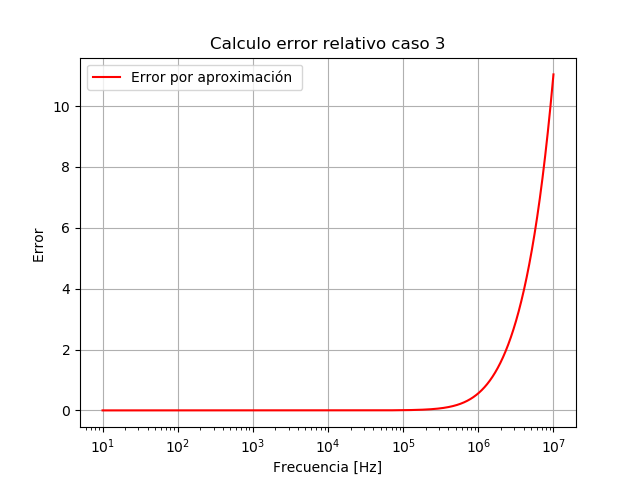
\includegraphics[width=\textwidth]{Ejercicio1/Imagenes/error3.png}
	\caption{Error relativo por aproximar Caso 3.}
	\label{fig:e3}
\end{figure}

De estos, es posible concluir que se puede utilizar la aproximación ideal siempre y cuando se tengan en cuenta la frecuencia de trabajo, y en caso de serlo necesario, el error que uno comete.

%%%%%%%%%%%%%%%%%%%%%%%%%%%%
\subsubsection{Calculo Analítico del Circuito No Inversor.}

De la misma forma que en el circuito inversor, se decidió aplicar el teorema de Thevenin.

\begin{figure}[H]
\begin{center}
\begin{circuitikz}
	\node [op amp](A1){};
	\draw (A1.-) to[short] ++(-1,0) to[R, l_=$R_1$] ++(-1.5,0) to[short] ++(-0.5,0) node[ground]{};
	\draw (A1.-) node[label=south:$V^-$]{};
	\draw (A1.+) node[label=south:$V^+$]{};
	\draw (A1.-) to[short] ++(0,1.5) to[R, l = $R_2$, i<_= $I_f$] ++(3,0) to[short] ++(0,-2);
	\draw (A1.out) to[short, -o] ++(1,0) node[ocirc,label=right:$V_{out}$]{};
	\draw (A1.+) to[short] ++(-1,0) to[R, l= $R_{Thevenin}$] ++(-1.5,0) to[short, -o] node[ocirc,label=left:$V_{Thevenin}$]{} ++(-0.5,0);
	\end{circuitikz}
	\caption{Equivalente de Thevenin del circuito inversor.}
	\label{fig:noinvThevenin}
\end{center}
\end{figure}

Siendo 
\begin{align}
	V_{Thevenin} = V_{in} \cdot \frac{R_4}{R_4+R_3} \\
	R_{Thevenin} = \frac{R_4\cdot R_3}{R_4+R_3}
\label{eq:noinvthev}
\end{align} 

Utilizando (\ref{equ:avoligualvo}) y planteando además

\begin{equation}
	V^+ = V_{Thevenin}
	\label{equ:noinvv+}
\end{equation}

\begin{equation}
	V^- = I_f R_1
\end{equation}

\begin{equation}
	V_{out} - I_f R_1 = V^-
\end{equation}

y operando algebraicamente, se puede demostrar que

\begin{equation}
	H \left(s \right) =\frac{A_{0}}{R_3} \cdot	\frac{R_3 // R_4}{1 \ + \ A_{0} \frac{R_1 // R_2}{R_2} } \cdot \left[ \frac{s}{\omega' \cdot \left( 1 + A_{0} \frac{R_1 // R_2}{R_2} \right)}  \ + \ 1 \right]^{-1}
	\label{equ:noinvtransferencia}
\end{equation}

considerando para este caso (\ref{eq:PoloDom}).

Para el caso de $A_{Vol}$ finito simplemente basta tomar:

\begin{equation}
	\lim_{\omega'\to\infty} H \left(s \right) =\frac{A_{0}}{R_3} \cdot	\frac{R_3 // R_4}{1 \ + \ A_{0} \frac{R_1 // R_2}{R_2} } \cdot \left[ \frac{s}{\omega' \cdot \left( 1 + A_{0} \frac{R_1 // R_2}{R_2} \right)}  \ + \ 1 \right]^{-1}
\end{equation}

Resultando en:

\begin{equation}
	H_{A_{vol}\space fin}\left(s \right) =\frac{A_{0}}{R_3} \cdot	\frac{R_3 // R_4}{1 \ + \ A_{0} \frac{R_1 // R_2}{R_2} }
	\label{equ:noinvtransferencia_avolfinito}
\end{equation}

Por otro lado, para $A_{Vol}$ finito solamente basta tomar:

\begin{align}
	\lim_{A_{vol}\to\infty} H_{A_{vol}=\infty} \left(s \right) = \frac{R_3 // R_4}{R_3} \cdot \frac{R_2}{R_1 // R_2}
\end{align}

Resultando en:

\begin{align}
	H_{A_{vol}=\infty} \left(s \right) = \frac{R_3 // R_4}{R_3} \cdot \frac{R_2}{R_1 // R_2}
		\label{equ:noinvtransferencia_ideal}
\end{align}

De (\ref{equ:noinvtransferencia}) se tiene que

\begin{equation}
	f_c = \frac{\omega'}{2 \pi}\cdot \left( 1 + A_{0} \frac{R_1 // R_2}{R_2} \right)
\end{equation}

Reemplazando con los valores presentados en la Tabla (\ref{tabla:resasignadas}), se puede recrear la Tabla (\ref{tabla:gananciasinv}) para el caso del circuito no inversor.

\begin{table}[H]
\begin{center}
\begin{tabular}{|c|c|c|c|}
\hline
\textbf{Caso}            & \textbf{1} & \textbf{2} & \textbf{3} \\ \hline
\textbf{$H(s)_{\infty}$} & $8.8$         & $1.6$          & $0.88$        \\ \hline
\textbf{$H(s)_{Finito}$} & $8.8$     & $1.6$     & $0.88$     \\ \hline
\textbf{$f_c$}           & $90.92 \ kHz$   & $500.01 \ kHz$  & $909.1 \ kHz$     \\ \hline
\end{tabular}
\caption{Ganancias y frecuencias de corte de los circuitos no inversores.}
\end{center}
\end{table}

De esta forma, se procede a comparar la transferencia para cada una de las consideraciones tenias en cuenta.

\begin{figure}[H]	
	\centering
	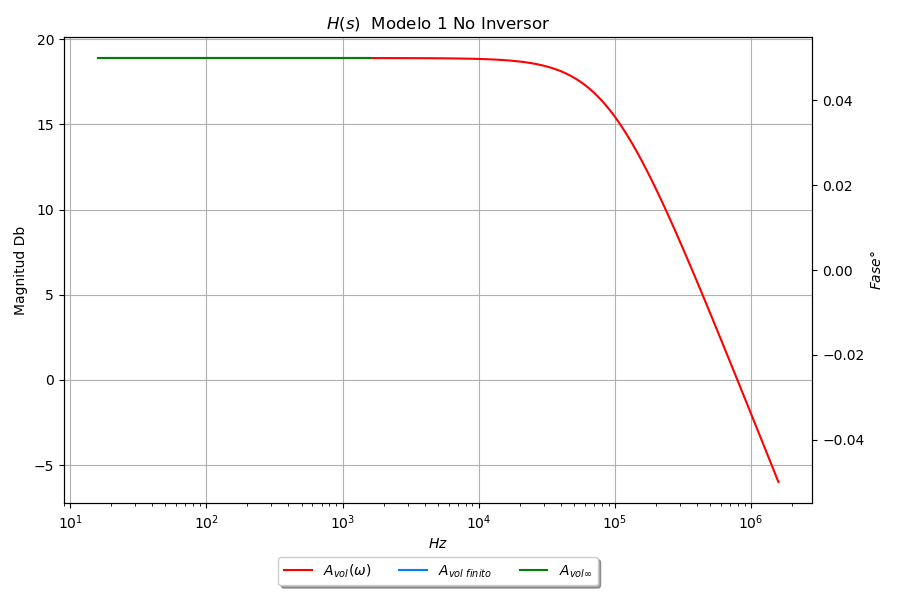
\includegraphics[width=\textwidth]{Ejercicio1/Imagenes/HCompC1_noinv.png}
	\caption{$H(s)$ para el Caso 1.}
	\label{fig:AvolC1_noinv}
\end{figure}

\begin{figure}[H]	
	\centering
	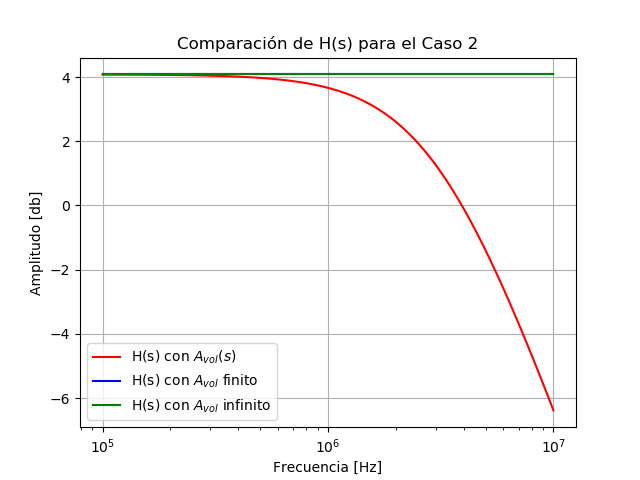
\includegraphics[width=\textwidth]{Ejercicio1/Imagenes/HCompC2_noinv.png}
	\caption{$H(s)$ para el Caso 2.}
	\label{fig:AvolC2_noinv}
\end{figure}

\begin{figure}[H]	
	\centering
	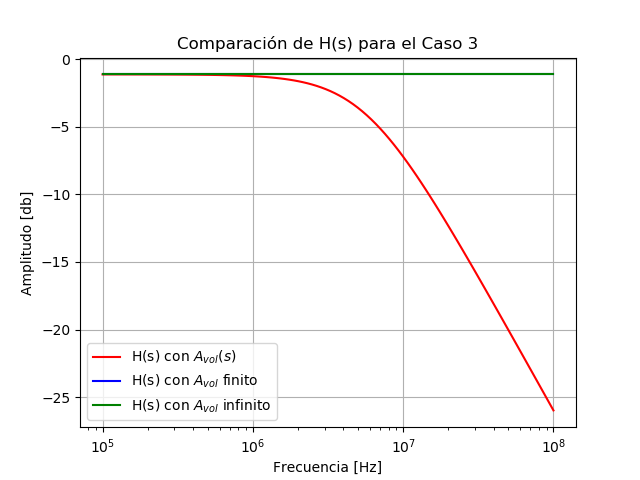
\includegraphics[width=\textwidth]{Ejercicio1/Imagenes/HCompC3_noinv.png}
	\caption{$H(s)$ para el Caso 3.}
	\label{fig:AvolC3_noinv}
\end{figure}

De igual forma que se realizó con el circuito inversor, se emplea (\ref{equ:error}) para calcular el error al considerar $A_{vol} (s)$ frente a $A_{vol \infty}$ en los distintos casos.

\begin{figure}[H]	
	\centering
	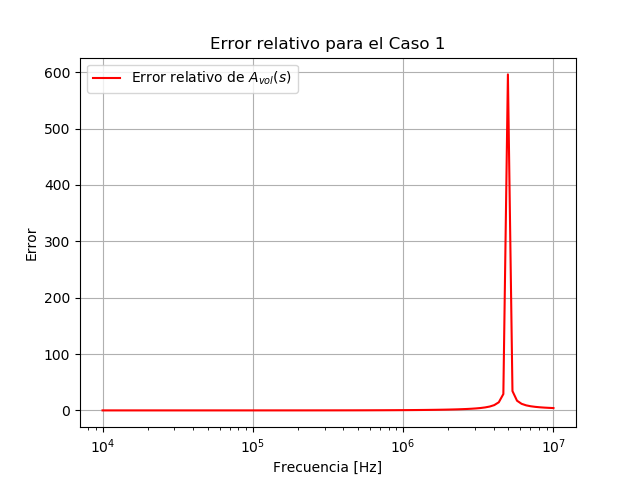
\includegraphics[width=\textwidth]{Ejercicio1/Imagenes/error1_noinv.png}
	\caption{Error relativo por aproximar $A_{vol}(s)$ para el Caso 1.}
\end{figure}
\begin{figure}[H]	
	\centering
	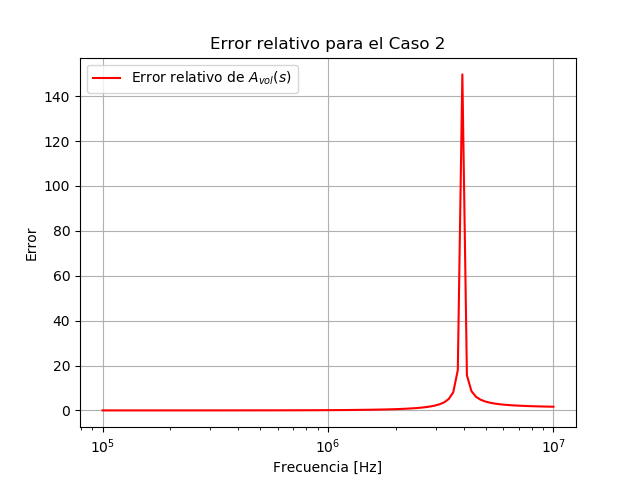
\includegraphics[width=\textwidth]{Ejercicio1/Imagenes/error2_noinv.png}
	\caption{Error relativo por aproximar $A_{vol}(s)$ para el Caso 2.}
\end{figure}
\begin{figure}[H]	
	\centering
	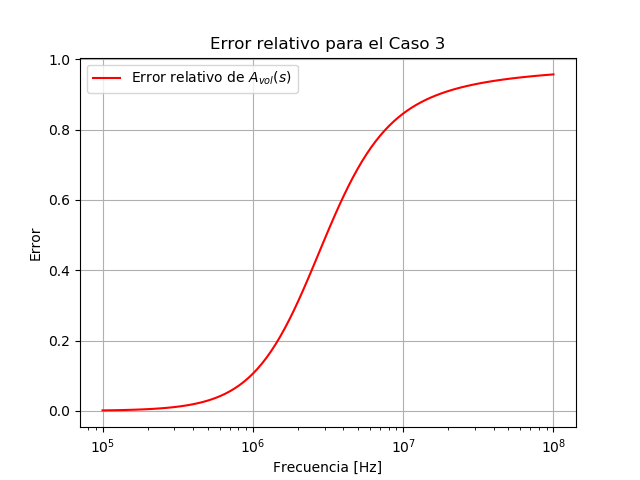
\includegraphics[width=\textwidth]{Ejercicio1/Imagenes/error3_noinv.png}
	\caption{Error relativo por aproximar $A_{vol}(s)$ para el Caso 3.}
\end{figure}

%%%%%%%%%%%%%%%%%%%%%%%%%%%%%%%%%%%%%%%%%%
\subsubsection{Impedancia de entrada.}

Para calcular la impedancia de entrada de los casos presentados se sigue la misma idea de la primer parte.

Se procede a analizar el caso del inversor. Sabiendo que
\begin{align}
\label{eq:Zin}
\frac{V_{Th} - V^-}{R_{Th}}=I_{in}
\end{align}
y ademas, utilizando (\ref{eq:thev}), (\ref{eq:nodeInv}) y (\ref{eq:Vout}), se puede llegar a la siguiente expresión:
\begin{align}
	Z_{in}(s)=\frac{A_{Vol}R_1R_3+R_1R_2+R_2R_3+R_1R_3}{A_{Vol}R_3+R_2+R_3}\cdot \frac{1+\frac{s\cdot (R_1R_2+R_1R_3+R_2R_3)}{\omega ' \cdot (A_{Vol}R_1R_3+R_1R_2+R_1R_3+R_2R_3)}}{1+\frac{s\cdot (R_2+R_3)}{\omega ' \cdot(A_{Vol}R_3+R_2+R_3)}}
\end{align}

También se puede observar en (\ref{eq:Zin}) que si $A_{Vol}$ es infinito, se cumple
\begin{align} V^- = V^+=0 \implies Z_{in}=R_1
\end{align}

Por otro lado, planteando de forma similar para el no inversor:
\begin{align}
\label{eq:noinvZin}
\frac{V_{Th} - V^+}{R_{Th}}=I_{in}
\end{align}
y valiendose del uso de (\ref{equ:noinvv+}), se llega a

\begin{equation}
	Z_{in} = R_3 + R_4
	\label{equ:zinnoinv}
\end{equation}

Las mediciones de la impedancia de entrada se realizaron de la siguiente manera:

\begin{center}
\begin{circuitikz}[american voltages] \draw (0,0)
  node[draw,minimum width=2cm,minimum height=2.4cm] (load) {Load}
  ($(load.west)!0.75!(load.north west)$) coordinate (la)
  ($(load.west)!0.75!(load.south west)$) coordinate (lb)
  (lb) to[short,-o] ++(-0.5,0) coordinate (b) node[ground]{}
  to[short] ++(-4,0) coordinate (VThb);
  \draw (VThb |- la) to[sV, v_=$V_{In}$] (VThb);
  \draw (VThb |- la)
  to[R=$R$] ++(2.5,0) coordinate (VTht)
  to[short,-o,i=$I_{In}$] (VTht -| b) coordinate (a) node[above] {$A$}
  to[short] (la);
  \path (a) node[below] {$+$} -- node {$V$} (b) node[above] {$\vphantom{+}-$};
\end{circuitikz}
\end{center}

Se optó por medir la de entrada la señal y la existente en el punto A, para poder emplear la de resta de ellas mediante el modo ``math'' del osciloscopio. Luego, se observó la proporción en decibeles y la fase, tanto de la resta como de la entrada, obteniendo las medidas correspondientes a la siguiente expresión:
\begin{align}
20\log\left(\frac{V_{(A-In)}}{V_{in}}\right)
\end{align}

A partir de estos valores se puede obtener la impedancia de entrada de la forma:

\begin{align}
Z_{In}=20\log\left(\frac{V_{In}}{I_{in}}\right) =20\log\left(\frac{V_{In} \cdot  R}{V_{(A-In)}}\right) = -20\log\left(\frac{V_{(A-In)}}{V_{In} }\right)+20\log (R)
\end{align}
para la fase con medir simplemente con medir la diferencia de fase entre la señal de entrada y la que cae sobre la resistencia es equivalente a medir la de la corriente  de entrada y la tensión de entrada dado a que la corriente sobre la resistencia y la caida de tensión sobre ella tienen la misma fase.


Luego se realizaron mediciones de la impedancia de entrada. De esta forma se compararon con simulaciones realizadas en LTSpice y con el calculo analítico. Cabe aclarar que para los gráficos, al realizar el calculo analítico, no fueron tomadas en cuentas las puntas del osciloscopio, las cuales se emplearon en modo \textbf{x1}, de forma que alteraron la medición, mientras que en las simulaciones con LTSpice si fueron tomadas en cuenta.

A continuación se presentan dichas medidas para el circuito inversor.

\begin{figure}[H]	
	\centering
	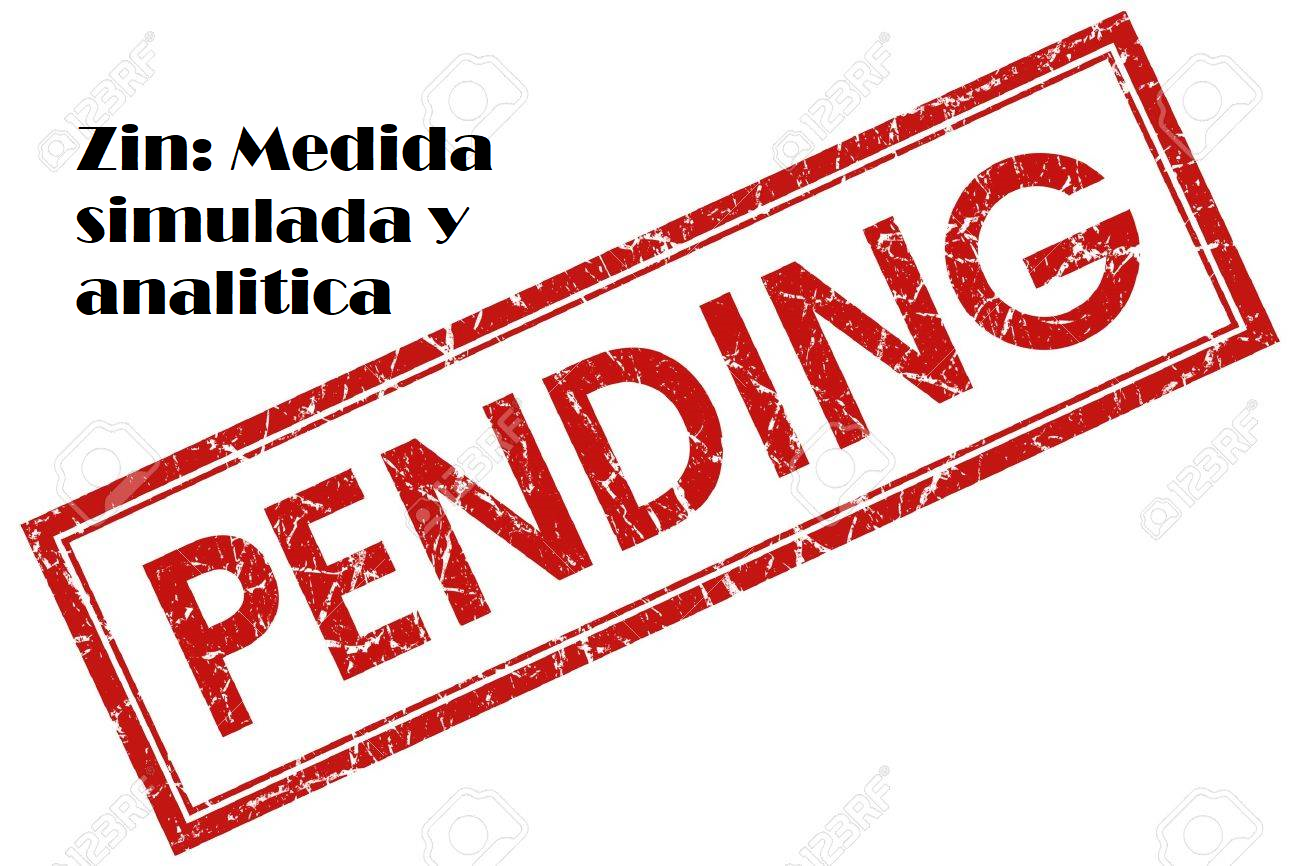
\includegraphics[width=0.9\textwidth]{Ejercicio1/Imagenes/ZinC1.png}
	\caption{BODE en modulo para el Caso 1 del circuito inversor.}
	\label{fig:CompZinC1inv}
\end{figure} 

\begin{figure}[H]	
	\centering
	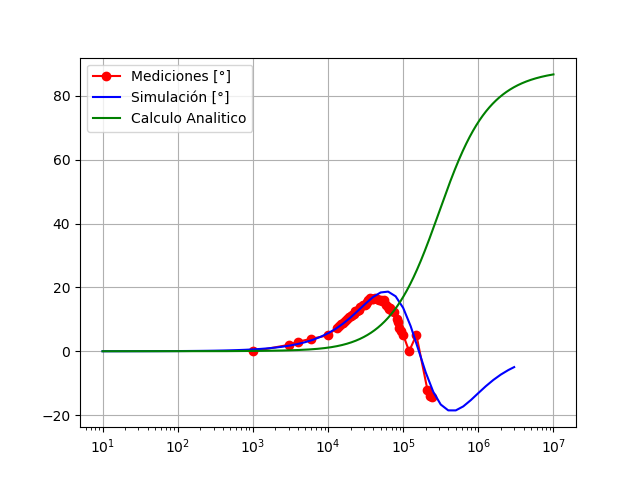
\includegraphics[width=0.9\textwidth]{Ejercicio1/Imagenes/ZinphC1.png}
	\caption{BODE en fase para el Caso 1 del circuito inversor.}
	\label{fig:CompZinphC1inv}
\end{figure} 

\begin{figure}[H]	
	\centering
	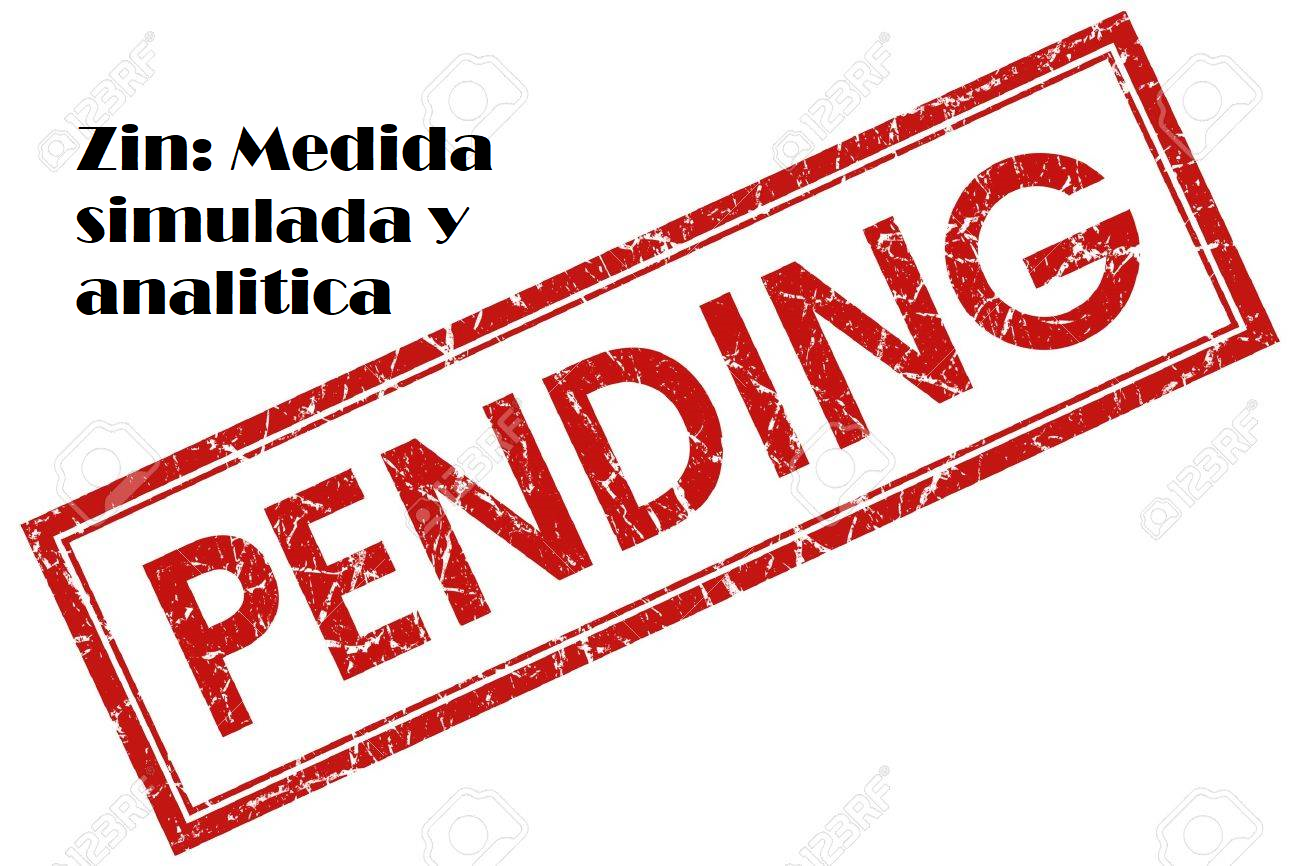
\includegraphics[width=0.9\textwidth]{Ejercicio1/Imagenes/CZinC2.png}
	\caption{BODE en modulo para el Caso 2 del circuito inversor.}
	\label{fig:CompZinC2inv}
\end{figure} 

\begin{figure}[H]	
	\centering
	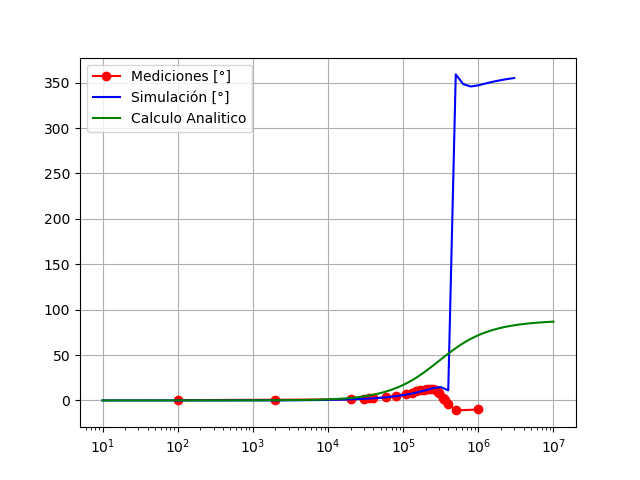
\includegraphics[width=0.9\textwidth]{Ejercicio1/Imagenes/ZinphC2.png}
	\caption{BODE en fase para el Caso 2 del circuito inversor.}
	\label{fig:CompZinphC2inv}
\end{figure} 

\begin{figure}[H]	
	\centering
	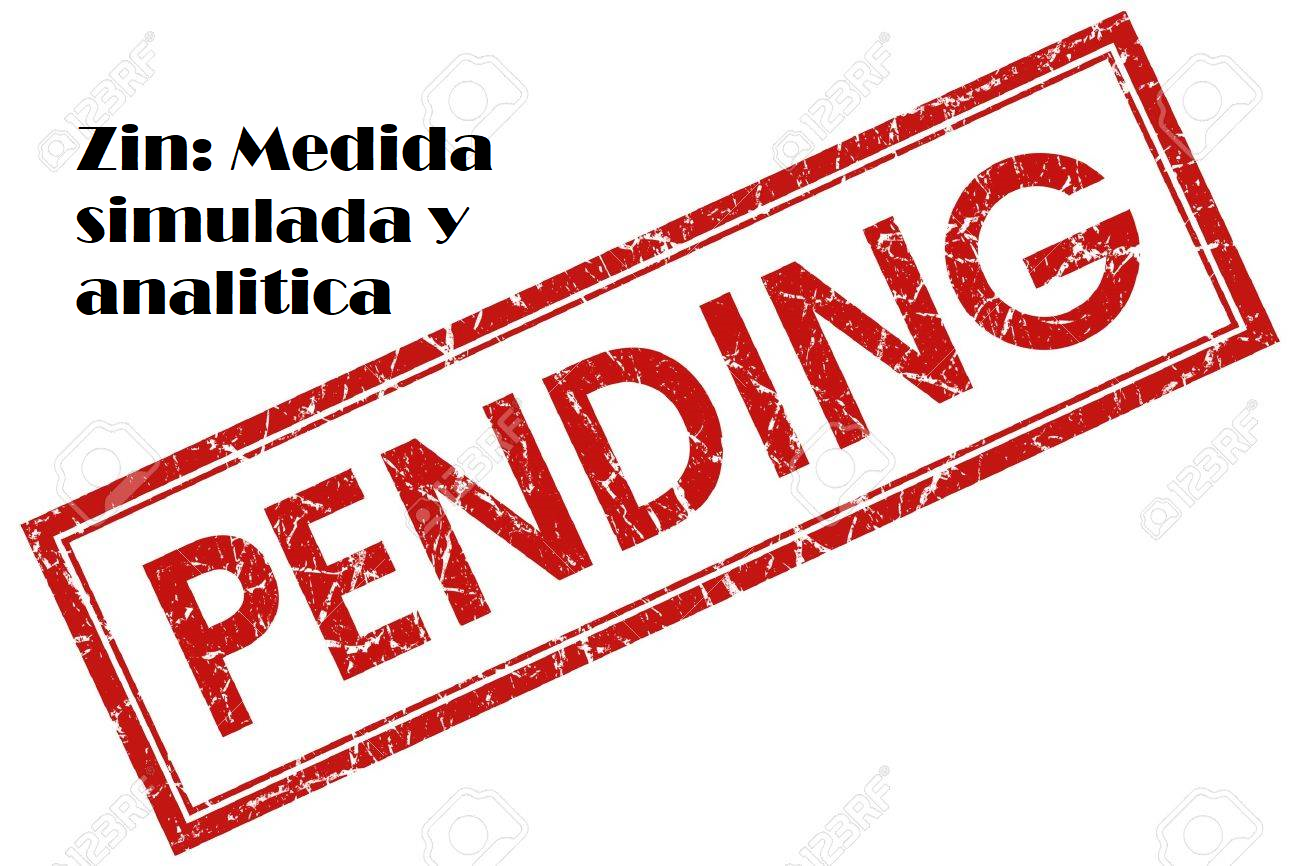
\includegraphics[width=\textwidth]{Ejercicio1/Imagenes/CZinC3.png}
	\caption{BODE en modulo para el Caso 3 del circuito inversor.}
	\label{fig:CompZinC3inv}
\end{figure} 

\begin{figure}[H]	
	\centering
	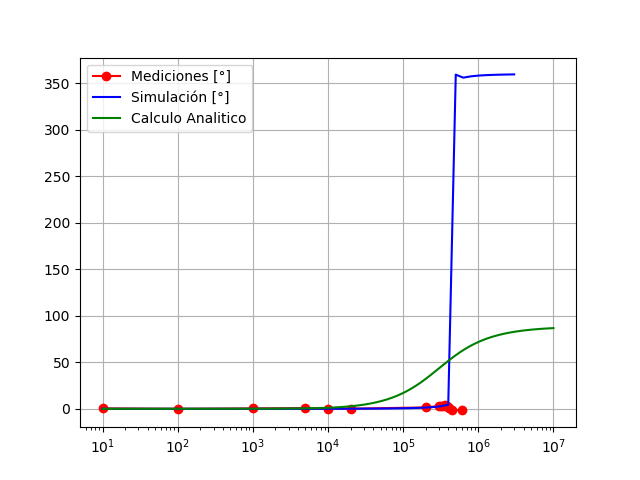
\includegraphics[width=\textwidth]{Ejercicio1/Imagenes/ZinphC3.png}
	\caption{BODE en fase para el Caso 3 del circuito inversor.}
	\label{fig:CompZinphC3inv}
\end{figure}

También cabe destacar que en las Figuras (\ref{fig:CompZinphC2inv}) y (\ref{fig:CompZinphC3inv}) realmente no hay un salto, sino que es un cambio de fase de $360^{\circ}$.

Luego se procede a mostrar las mediciones realizadas para el caso del circuito no inversor.

\begin{figure}[H]	
	\centering
	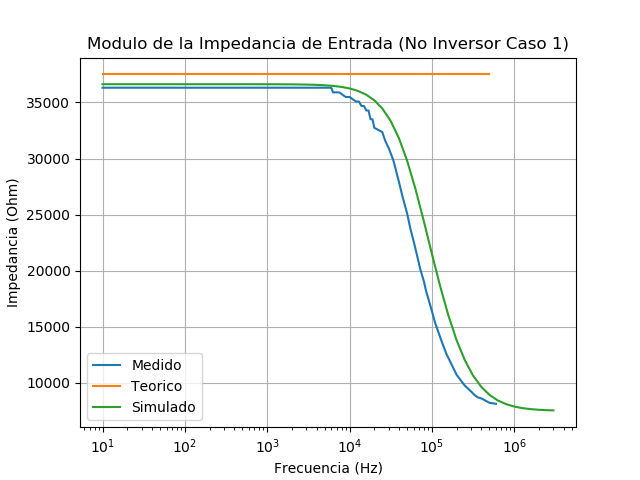
\includegraphics[width=0.9\textwidth]{Ejercicio1/Imagenes/ZinC1_Noinv.png}
	\caption{BODE en modulo para el Caso 1 del circuito no inversor.}
	\label{fig:NoInvCompZinC1}
\end{figure} 

\begin{figure}[H]	
	\centering
	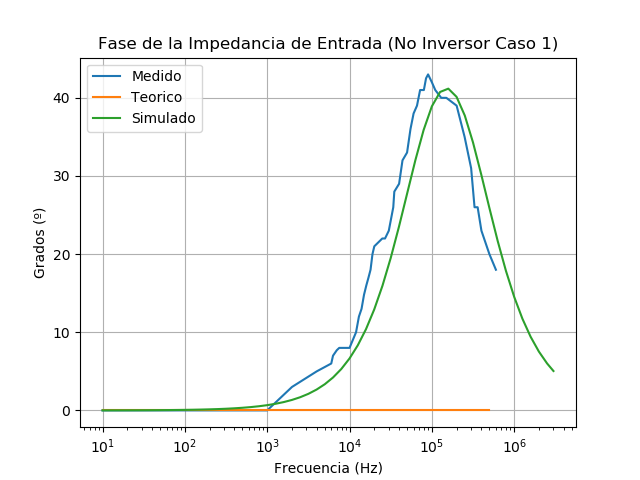
\includegraphics[width=0.9\textwidth]{Ejercicio1/Imagenes/ZinphC1_Noinv.png}
	\caption{BODE en fase para el Caso 1 del circuito no inversor.}
	\label{fig:NoInvCompZinphC1}
\end{figure} 

\begin{figure}[H]	
	\centering
	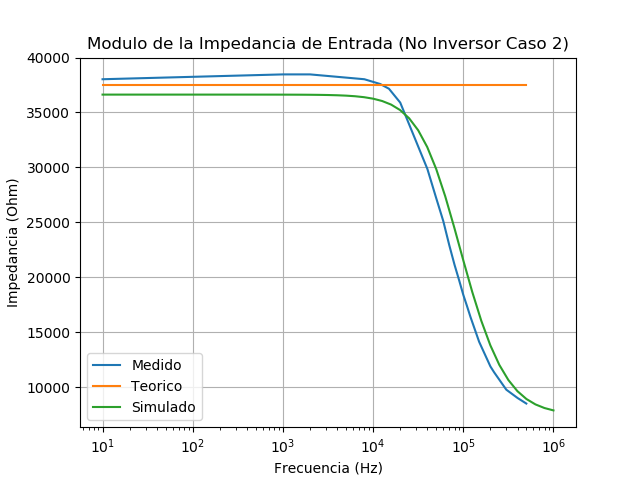
\includegraphics[width=0.9\textwidth]{Ejercicio1/Imagenes/ZinC2_Noinv.png}
	\caption{BODE en modulo para el Caso 2 del circuito no inversor.}
	\label{fig:NoInvCompZinC2}
\end{figure} 

\begin{figure}[H]	
	\centering
	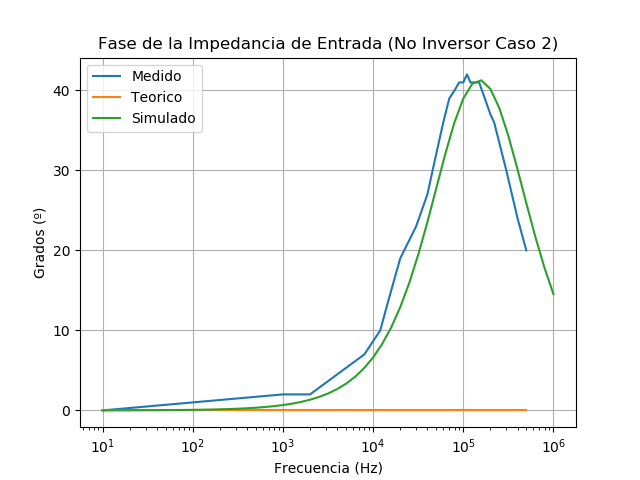
\includegraphics[width=0.9\textwidth]{Ejercicio1/Imagenes/ZinphC2_Noinv.png}
	\caption{BODE en fase para el Caso 2 del circuito no inversor.}
	\label{fig:NoInvCompZinphC2}
\end{figure} 

\begin{figure}[H]	
	\centering
	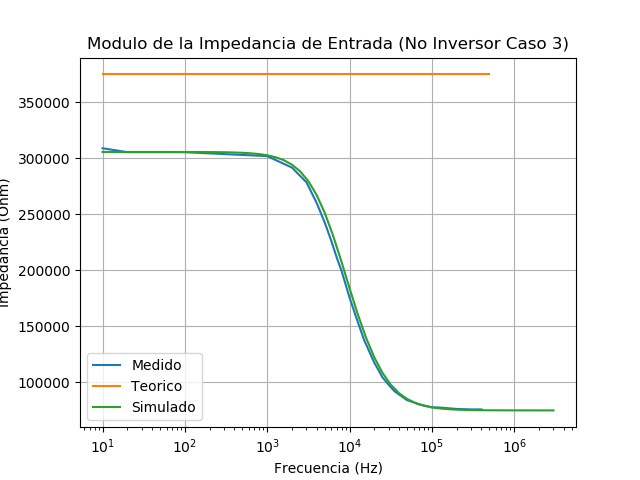
\includegraphics[width=\textwidth]{Ejercicio1/Imagenes/ZinC3_Noinv.png}
	\caption{BODE en modulo para el Caso 3 del circuito no inversor.}
	\label{fig:NoInvCompZinC3}
\end{figure} 

\begin{figure}[H]	
	\centering
	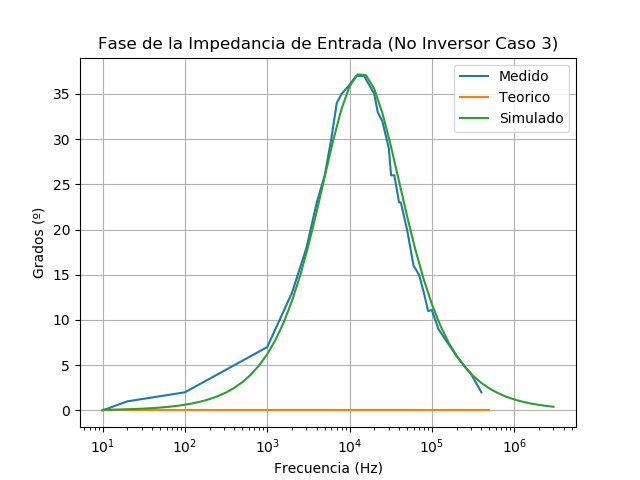
\includegraphics[width=\textwidth]{Ejercicio1/Imagenes/ZinphC3_Noinv.png}
	\caption{BODE en fase para el Caso 3 del circuito no inversor.}
	\label{fig:CompZinphC3}
\end{figure}

%%%%%%%%%%%%%%%%%%%%%%%%%%%%%%
\subsubsection{Máximos valores de entrada.}

\begin{center}
\textcolor{red}{\textbf{VER PARA EL NO INVERSOR.}}
\textcolor{red}{\textbf{HACER LAS CUENTAS Y LOS GRÁFICOS.}}
\end{center}

El máximo valor de entrada a partir del cual el opamp satura se encuentra definido por diversas variables, siendo algunas de ellas la ganancia del sistema, la amplitud y la frecuencia de la entrada.

Al momento de definir los valores posibles, se realizó un enfoque en las tres variables previamente mencionadas y se asumió el opamp con ganancia ideal. Cabe recordar que se empleó la formula $ V_{Out}=H(s)\cdot V_{in} $.

De esta forma, el máximo valor de $V_{in}$ queda definido por la tensión de saturación del operacional. Para el utilizado en este informe (LM324), dicho valor es de $Vcc - 1.5 \ V$\footnote{Dato extraído de la hoja de datos.}, siendo así, para el caso empleado, equivalente a $13.5 \ V$. Luego, utilizando esta relación, se plasmaron los resultados, para las distintas ganancias analizadas, en la Tabla (\ref{tab:gananciaideal}). Cabe descara que para el caso 3 se realiza una excepción, ya que el fabricante informa que la máxima tensión de entrada soportada por el dispositivo sin quemarse es de $32 \ V$.

\begin{table}[H]
\begin{center}
\label{tab:maxin}
\begin{tabular}{|c|c|c|c|}
\hline
\textbf{Caso}        & \textbf{1} & \textbf{2} & \textbf{3} \\ \hline
\textbf{Ganancia ideal}     & 10         & 1          & 0.1        \\ \hline
\textbf{$V_{in-Max} \ \left[ V \right]$} & 1.35       & 13.5       & 32         \\ \hline
\end{tabular}
\end{center}
\caption{Ganancia ideal para el operacional LM324.}
\label{tab:gananciaideal}
\end{table}

Luego se graficó la máxima tensión de entrada en función de la ganancia:
\begin{figure}[H]	
	\centering
	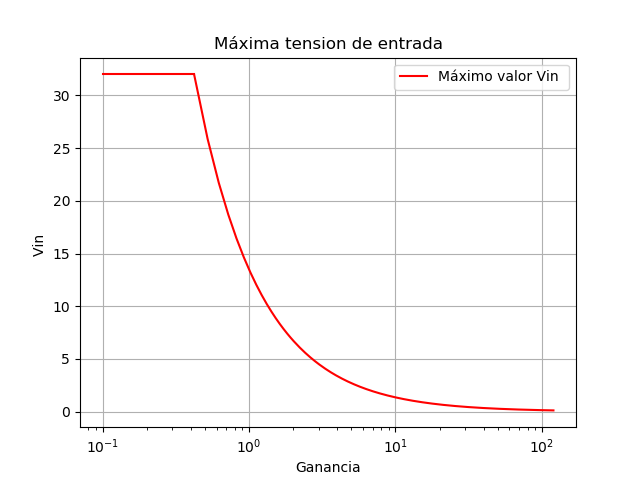
\includegraphics[width=\textwidth]{Ejercicio1/Imagenes/maxvin.png}
	\caption{Máxima tensión de entrada en función de la ganancia.}
	\label{fig:MaxVin}
\end{figure} 

También se analizó la máxima amplitud de entrada en función de la frecuencia tal que no haya Slew-Rate, el cual es un efecto que se detalla con mayor profundidad en su propia sección, ni saturación.
La cual puede ser apreciada en el siguiente gráfico:
\begin{figure}[H]	
	\centering
	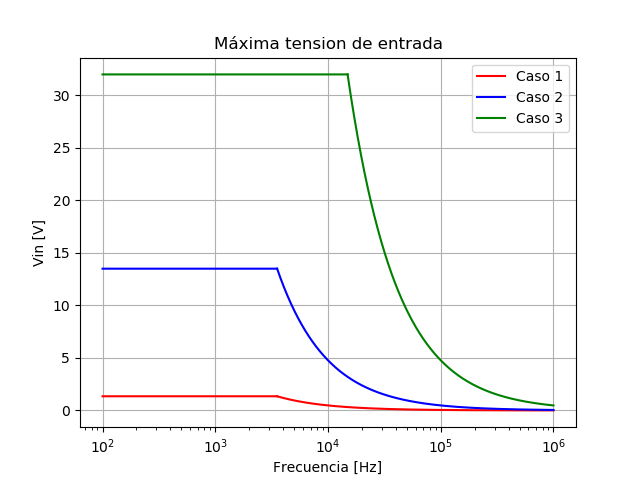
\includegraphics[width=\textwidth]{Ejercicio1/Imagenes/maxvinsr.png}
	\caption{Máxima tensión de entrada sin saturación ni Slew-Rate.}
	\label{fig:MaxVinsr}
\end{figure} 
%%%%%%%%%%%%%%%%%%
\subsubsection{Principales Características.}
En el caso del circuito inversor, considerando la situación en la cual $R_3$ sea igual a 0, la salida del amplificador operacional debería ser de $0 \ V$. Esto no es lo que ocurre dado que existe una tensión de offset, la cual se analiza en la sección 3 de este informe.

Por su parte, para el circuito no inversor, se obtendría que $V^+ = V_{in}$. Este circuito se caracteriza por poder ser sustentado con una sola fuente de alimentación, siendo esta referenciada a $V^+/2$ \footnote{Caracterización brindada por el fabricante.}. Es así que recalculando la ganancia para esta disposición, se obtiene que 
\[
	H \left(s \right) = \left( \frac{R_1}{R_1 + R_2} + A_o\left( \omega \right) \right)^{-1}
\]

Luego, se sabe que $R_3$ no es necesaria considerando $I_{in}$ constante frente a cambios en la temperatura\footnote{Dato obtenido de la hoja de datos}. Además, se observa en (\ref{equ:zinnoinv}) que la impedancia de entrada decae, lo cual puede llegar a provocar que esta sea comparable con la de la fuente, generando problemas de medición.

Por otro lado, se analiza el propósito de $R_4$ en el circuito inversor. A primera vista no es evidente, dado que la transferencia es independiente de ella, pero observando que existe una corriente máxima\footnote{Dato obtenido de la datasheet, $I_{Max}=20 \ mA$} que puede aportar el opamp, se llego a que el propósito de $R_4$ es limitar la corriente, por lo tanto su valor debe ser $R_4>\frac{V_{Out}}{I_{Max}}$. Otra función que posee $R_4$ es el limitar la corriente del lazo.
%%%%%%%%%%%%%%%%%%%%

\subsubsection{DC-Sweep.}
Se realizó un barrido entre $-Vcc$ y $Vcc$, utilizando un generador de funciones con una rampa y un circuito inversor para llegar a la tensión de salida necesitada, dado que el generador de funciones solo puede entregar hasta $20 \ Vpp$.
El comportamiento del operacional no es lineal para todo el rango de entradas. Este se puede observar únicamente en el rango entre $-V_{sat}$ y $V_{sat}$. Considerando las tensiones de entrada máxima que se observan en la Figura (\ref{fig:MaxVinsr}), se registraron las siguientes mediciones para el circuito inversor:

\begin{figure}[H]	
	\centering
	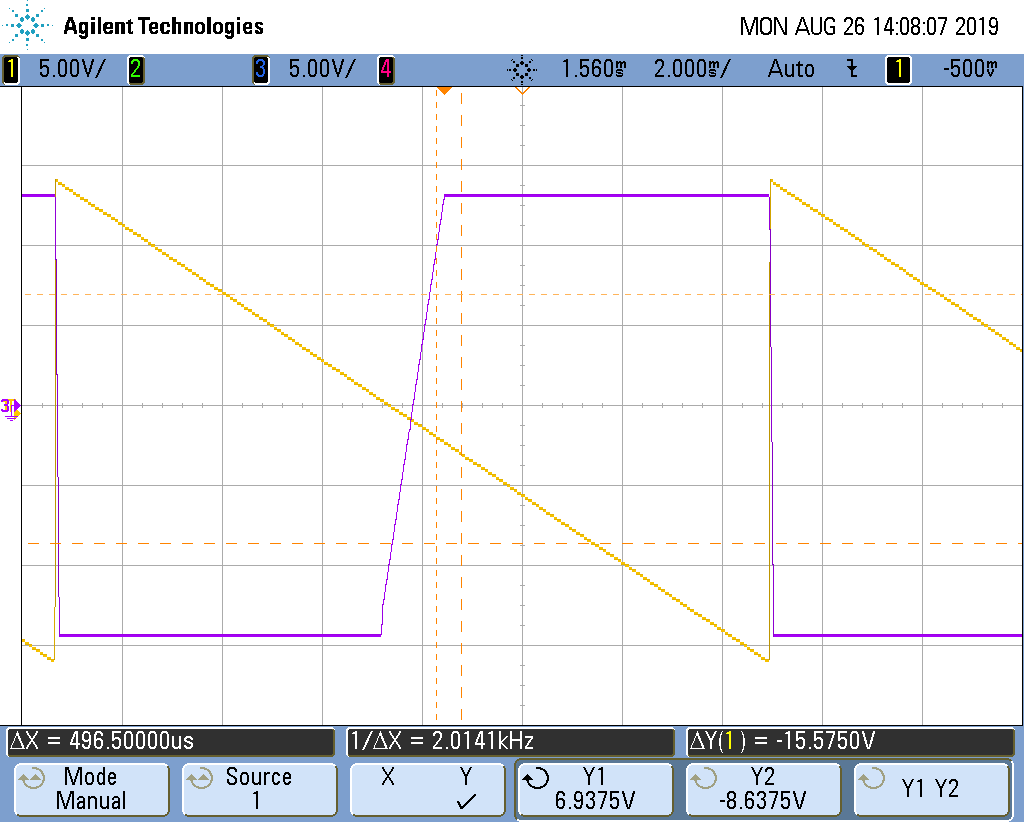
\includegraphics[width=0.8\textwidth, trim = {0 3.3cm 0 2cm},clip]{Ejercicio1/Imagenes/dc_sweep_c1.png}
	\caption{DC-sweep del circuito inversor, Caso 1.}
	\label{fig:dcc1}
\end{figure} 
Se puede observar en este caso como el opamp satura a partir de una tensión mayor a $1.35 V$ como se predijo en le punto (a).
\begin{figure}[H]	
	\centering
	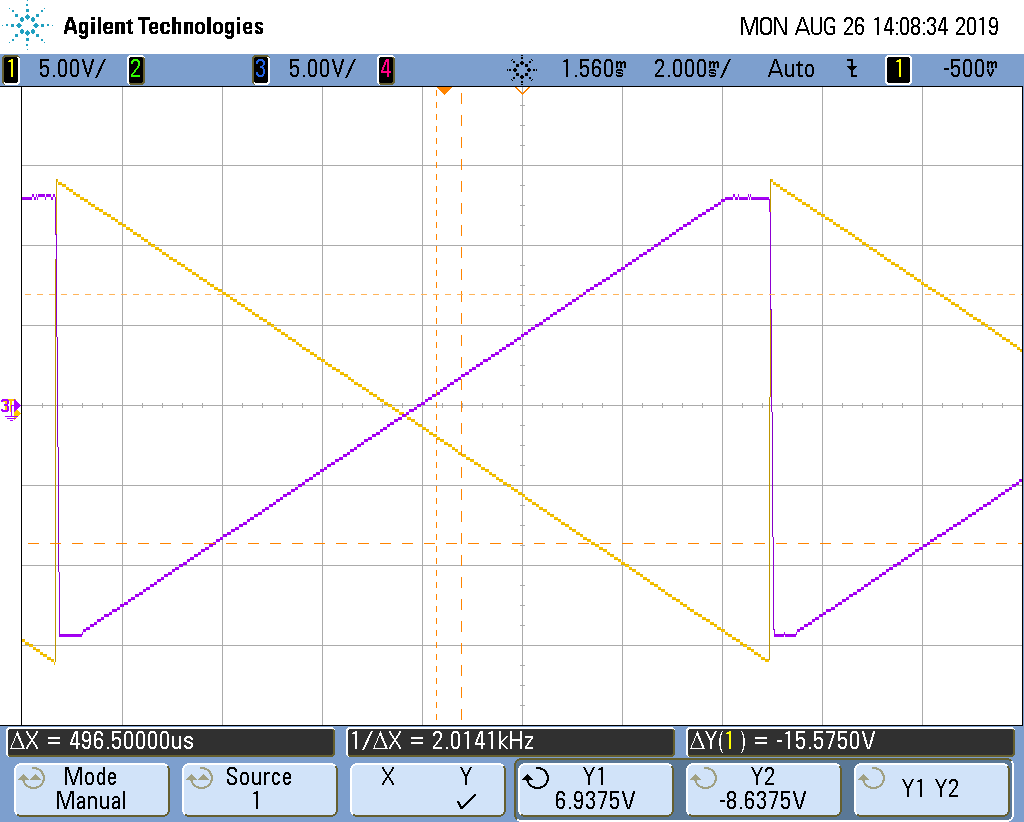
\includegraphics[width=0.8\textwidth, trim = {0 3.3cm 0 2cm},clip]{Ejercicio1/Imagenes/dc_sweep_c2.png}
	\caption{DC-sweep del circuito inversor, Caso 2.}
	\label{fig:dcc2}
\end{figure} 
En esta figura se ve como el comportamiento del amplificador operacional es lineal en la mayoría del espectro, con la excepción de las puntas, como fue explicado en el punto (a), para tensiones próximas a los $ 13.5 \ V$.
\begin{figure}[H]	
	\centering
	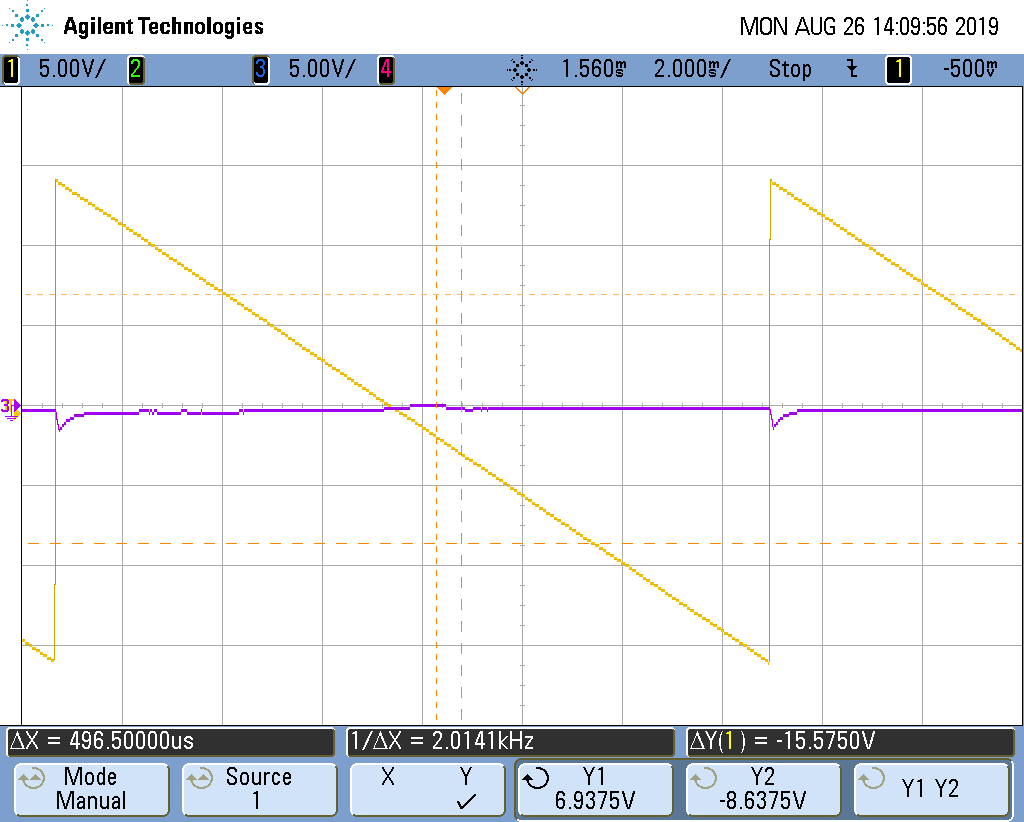
\includegraphics[width=0.8\textwidth, trim = {0 3.3cm 0 2cm},clip]{Ejercicio1/Imagenes/dc_sweep_c3.png}
	\caption{DC-sweep del circuito inversor, Caso 3.}
	\label{fig:dcc3}
\end{figure} 
Finalmente en esta figura se muestra que el opamp tiene comportamiento lineal para todos los valores de la rampa.

Luego, se procede a presentar el mismo análisis aplicado al circuito no inversor:

\begin{figure}[H]	
	\centering
	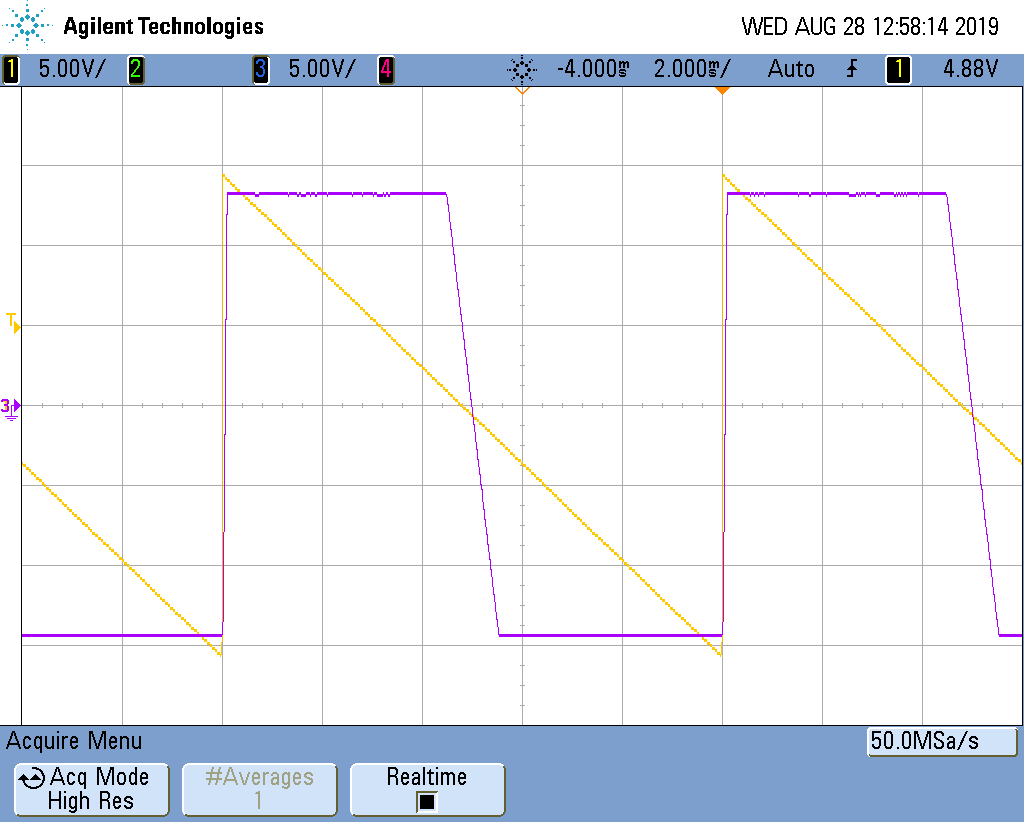
\includegraphics[width=0.8\textwidth, trim = {0 3.3cm 0 2cm},clip]{Ejercicio1/Imagenes/dc_sweep_c1_noinv.png}
	%trim={<left> <lower> <right> <upper>}
	\caption{DC-sweep del circuito no inversor, Caso 1.}
	\label{fig:dcc1noi}
\end{figure} 

\begin{figure}[H]	
	\centering
	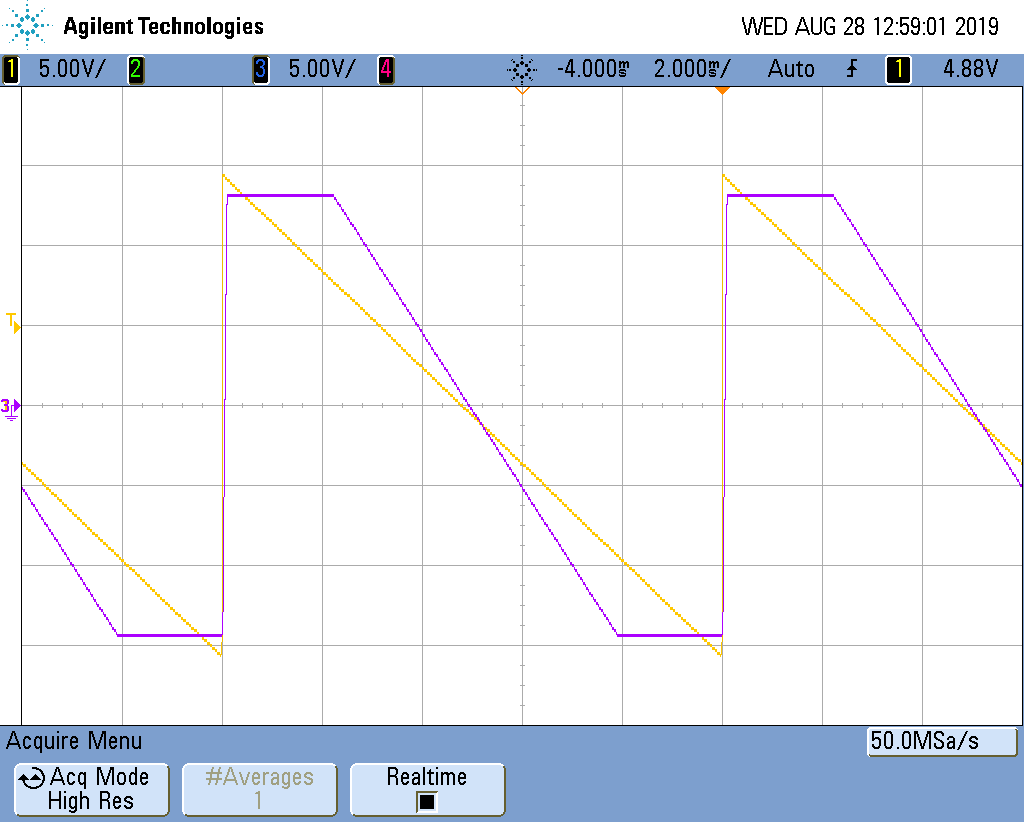
\includegraphics[width=0.8\textwidth, trim = {0 3.3cm 0 2cm},clip]{Ejercicio1/Imagenes/dc_sweep_c2_noinv.png}
	\caption{DC-sweep del circuito no inversor, Caso 2.}
	\label{fig:dcc2noi}
\end{figure} 

\begin{figure}[H]	
	\centering
	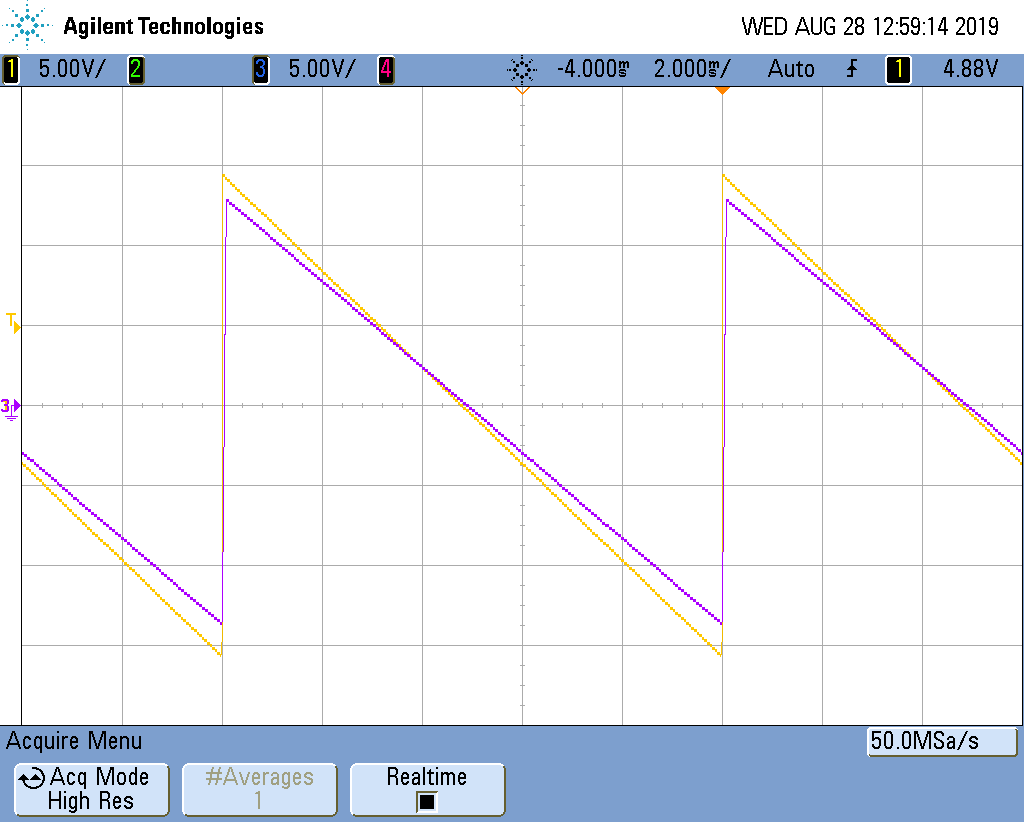
\includegraphics[width=0.8\textwidth, trim = {0 3.3cm 0 2cm},clip]{Ejercicio1/Imagenes/dc_sweep_c3_noinv.png}
	\caption{DC-sweep del circuito no inversor, Caso 3.}
	\label{fig:dcc3noi}
\end{figure} 

Los casos mostrados en las Figuras (\ref{fig:dcc1noi}), (\ref{fig:dcc2noi}) y (\ref{fig:dcc3noi}) son muy similares a los presentados en (\ref{fig:dcc1}), (\ref{fig:dcc2}) y (\ref{fig:dcc3}). Esto es un resultado esperable, ya que los ordenes con los cuales se amplifican las señales de entrada, para cada caso, son similares, provocando que las tensiones de saturación también lo sean, con la salvedad del cambio de signo en la tensión de entrada para cada tipo de circuito.

Otro efecto no lineal del amplificador operacional que fue observado es el efecto de Cross-Over, el cual es introducido dado a la polarización de los transistores que tiene por dentro el operacional. Este efecto se hace notar como una deformación en forma de llanura en la transición por $0 \ V$, como se puede apreciar en la Figura (\ref{fig:co}).

Se puede evitar tener que lidiar con este problema al aplicar una tensión de offset de continua, de forma tal que se consiga polarizar los transistores. Para ello, en este informe, se emplearon valores entre $0.7 \ V$ y $1.4 \ V$. Otra alternativa es valerse de una señal con valor medio mayor a $0.7 \ V$. 
\begin{figure}[H]	
	\centering
	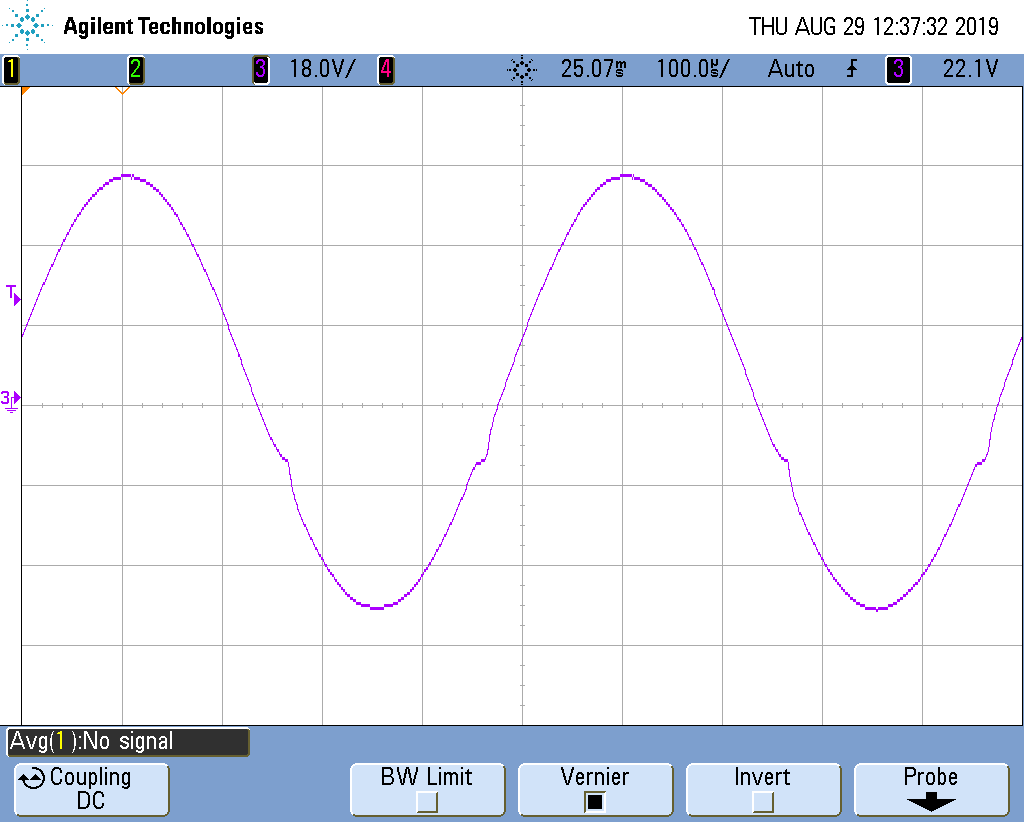
\includegraphics[width=0.8\textwidth, trim = {0 3.3cm 0 2cm},clip]{Ejercicio1/Imagenes/CrossOver.png}
	\caption{Señal con Cross-Over.}
	\label{fig:co}
\end{figure} 

%%%%%%%%%%%%%%%%%%%%%%%%%%
\subsubsection{Slew-Rate.}
El Slew-Rate está definido como la máxima variación temporal de la salida del amplificador operacional. Este efecto depende de 3 parámetros siendo estos la frecuencia, la amplitud y la ganancia, considerando el caso de que la salida sea una senoidal. Dado que se puede describir cualquier señal como una combinación lineal de senos, se puede decir que el Slew-Rate de una señal arbitraria también dependerá de estos parámetros. Si se le demanda al operacional una tasa de cambio mayor a la soportada, este procederá a distorsionar la señal.
\begin{align}
	SR= Max\left( \frac{\partial V_{Out}}{\partial t}\right)
\end{align}

Utilizando una entrada senoidal de la forma $V_{in}=A\cdot \sin (\omega t)$:
\begin{align}
	SR= Max\left( \frac{\partial (G\cdot A\cdot \sin (\omega t))}{\partial t}\right) = A \cdot \omega \cdot G  
\label{eq:sr}
\end{align}

A partir de (\ref{eq:sr}) se llega a una relación que debe cumplir la señal de entrada para no presentar efectos de Slew-Rate. Esta limitación tiene un grado de libertad, por lo tanto se puede elegir un parámetro fijo y regular el otro, por ejemplo, fijando la frecuencia de entrada, se deberá cumplir que:
\begin{align} V_{in}	\leq \frac{SR}{G\cdot \omega_0}\end{align}

Es así que se midió el Slew-Rate utilizando como entrada una senoidal, obteniendo la siguiente medición:
\begin{figure}[H]	
	\centering
	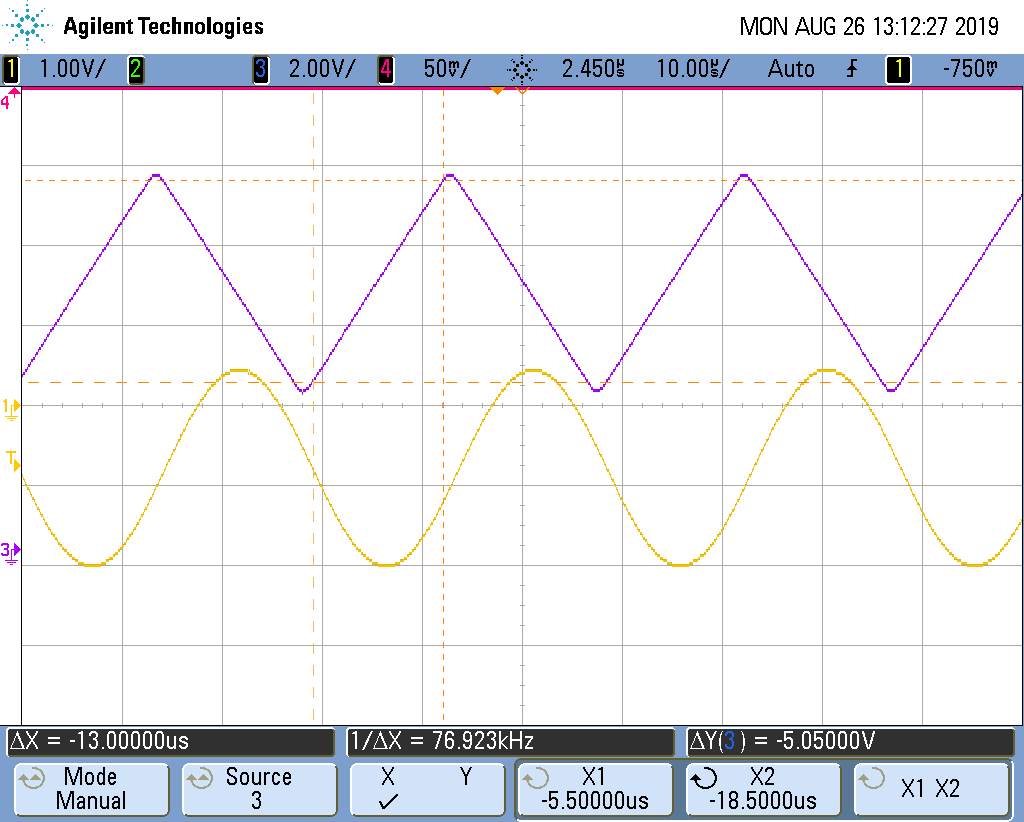
\includegraphics[width=0.8\textwidth, trim = {0 3.3cm 0 2cm},clip]{Ejercicio1/Imagenes/slew_rate1.png}
	\caption{Medición Slew-Rate.}
	\label{fig:SlewRate}
\end{figure}
De aqui utilizando (\ref{eq:sr}) se obtiene que:
\begin{align}
SR \approx  0.38 \frac{V}{\mu s}
\end{align}
lo cual concuerda con lo provisto por el fabricante en la Tabla (\ref{tab:datos}).
%%%%%%%%%%%%%%%%%%%%%%%%%%%%%%%%%%%%
\subsubsection{Respuesta en frecuencia.}
Se midió la respuesta en frecuencia de las configuraciones en los diversos casos y se graficaron junto a las simulaciones hechas en LTSpice y los cálculos teóricos.

Primero se presentan los casos para el circuito inverso.
\begin{figure}[H]	
	\centering
	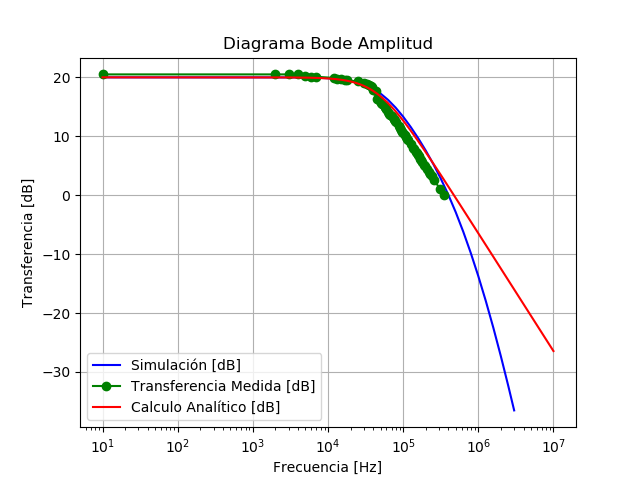
\includegraphics[width=0.8\textwidth]{Ejercicio1/Imagenes/BodeC1.png}
	\caption{Diagrama de Bode en amplitud Caso 1.}
	\label{fig:BodeC1}
\end{figure} 
\begin{figure}[H]	
	\centering
	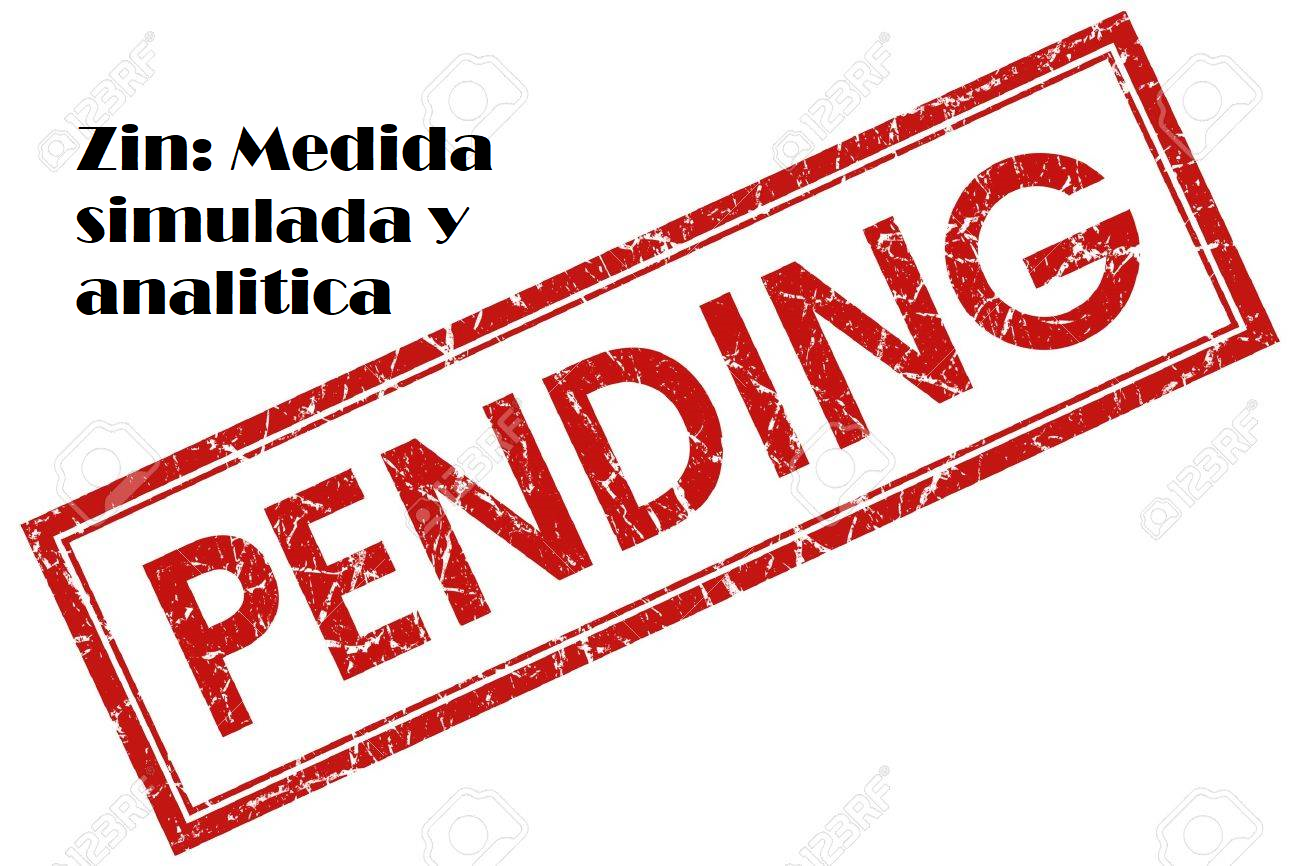
\includegraphics[width=0.8\textwidth]{Ejercicio1/Imagenes/BodephC1.png}
	\caption{Diagrama de Bode en fase Caso 1.}
	\label{fig:BodephC1}
\end{figure} 

En estas mediciones el principal problema que se presentó fue la saturación propia del operacional. También se evidenciaron los efectos del Slew-Rate dado a que esta configuración amplifica y efecto de Cross-Over. Además, se observó que, dado que la tensión de entrada era tan pequeña, como se puede apreciar en la Figura (\ref{fig:MaxVinsr}), la señal era comparable con ruido, el cual a su vez era amplificado y obteniendo uno mucho mayor a la salida.
\begin{figure}[H]	
	\centering
	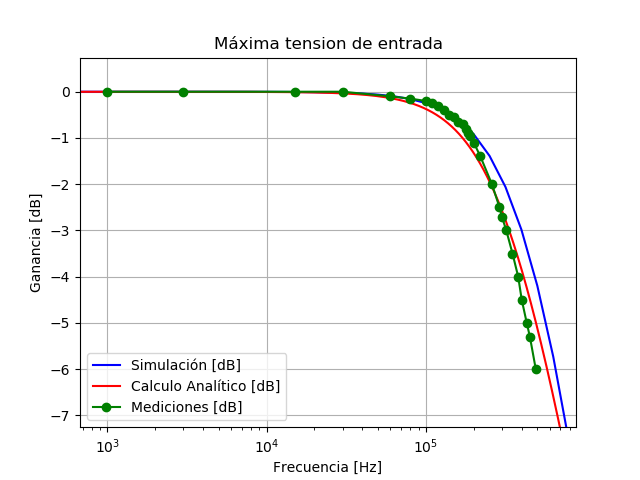
\includegraphics[width=0.8\textwidth]{Ejercicio1/Imagenes/BodeC2.png}
	\caption{Diagrama de Bode en amplitud Caso 2.}
	\label{fig:BodeC2}
\end{figure} 
\begin{figure}[H]	
	\centering
	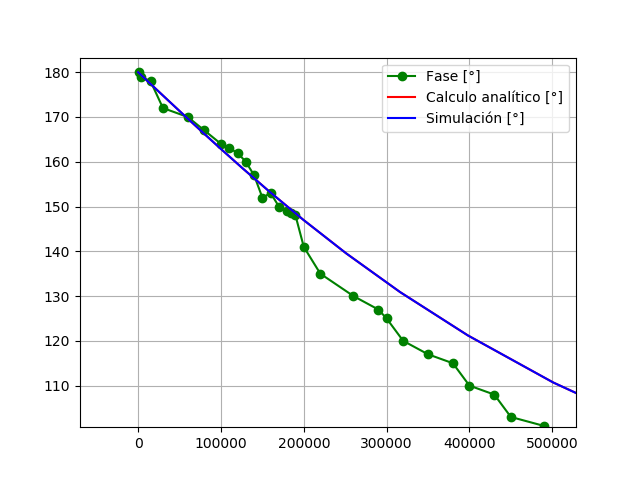
\includegraphics[width=0.8\textwidth]{Ejercicio1/Imagenes/BodephC2.png}
	\caption{Diagrama de Bode en fase Caso 2.}
	\label{fig:BodephC2}
\end{figure} 


\begin{figure}[H]	
	\centering
	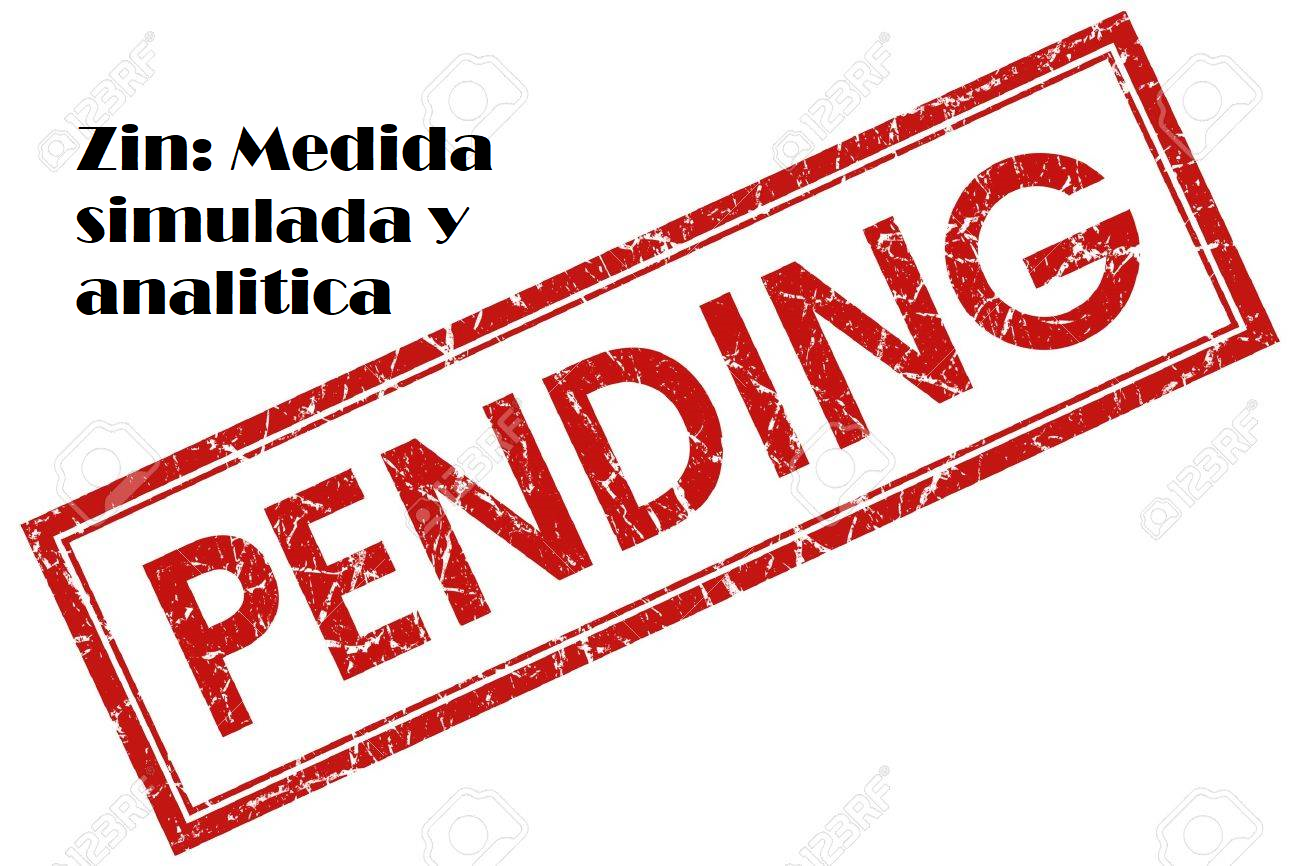
\includegraphics[width=0.8\textwidth]{Ejercicio1/Imagenes/BodeC3.png}
	\caption{Diagrama de Bode en amplitud Caso 3.}
	\label{fig:BodeC3}
\end{figure} 
\begin{figure}[H]	
	\centering
	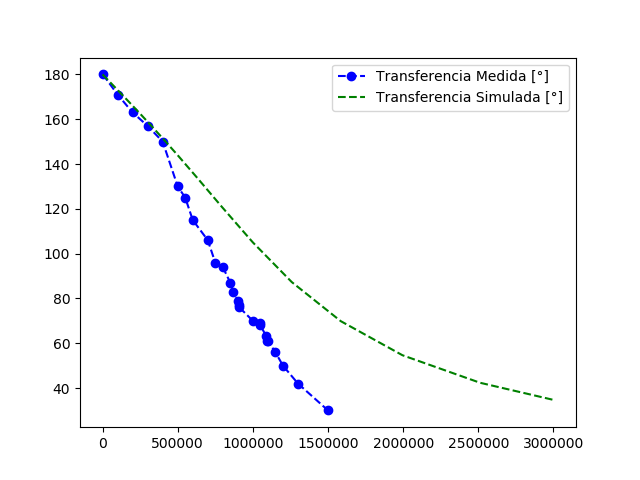
\includegraphics[width=0.8\textwidth]{Ejercicio1/Imagenes/BodephC3.png}
	\caption{Diagrama de Bode en fase Caso 3.}
	\label{fig:BodephC3}
\end{figure} 

Para las mediciones del tercer caso, se presentó el problema de que se dificultó la toma de mediciones, debido a que, se estaba atenuando la señal a medir, por lo tanto se encontraba cerca del piso de ruido a altas frecuencias. Algo que se puede apreciar en esta medición es la aparición de un sobrepico. Las mismas fueron hechas con una punta \textbf{x10}, la cual introdujo un polo adicional, generando un sistema de segundo orden, justificando la aparición de dicho sobrepico.

A continuación se presentan las mediciones realizadas para el circuito no inversor.

\begin{figure}[H]	
	\centering
	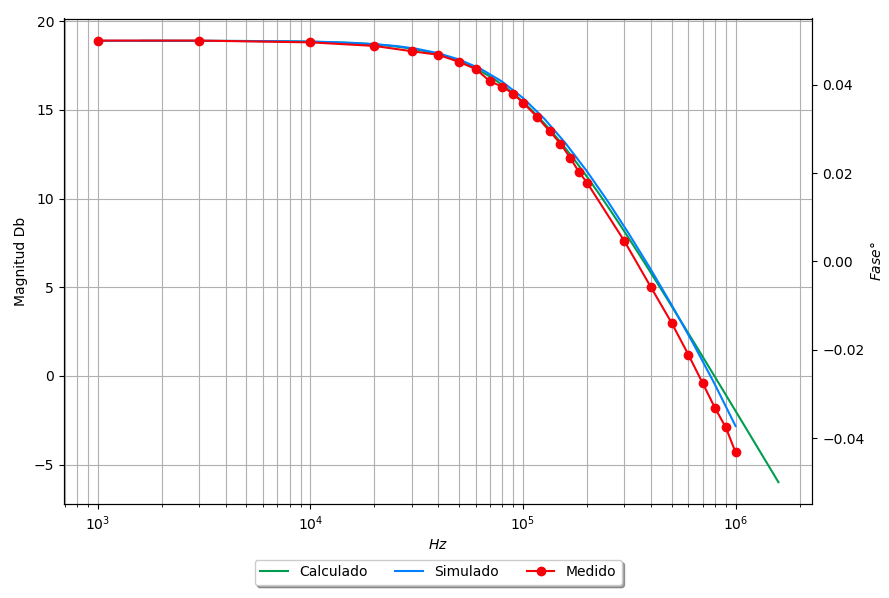
\includegraphics[width=0.8\textwidth, trim = {0 0 2cm 0},clip]{Ejercicio1/Imagenes/BodeC1_noinv.png}
	\caption{Diagrama de Bode en amplitud Caso 1.}
	\label{fig:BodeC1_noinv}
\end{figure} 
\begin{figure}[H]	
	\centering
	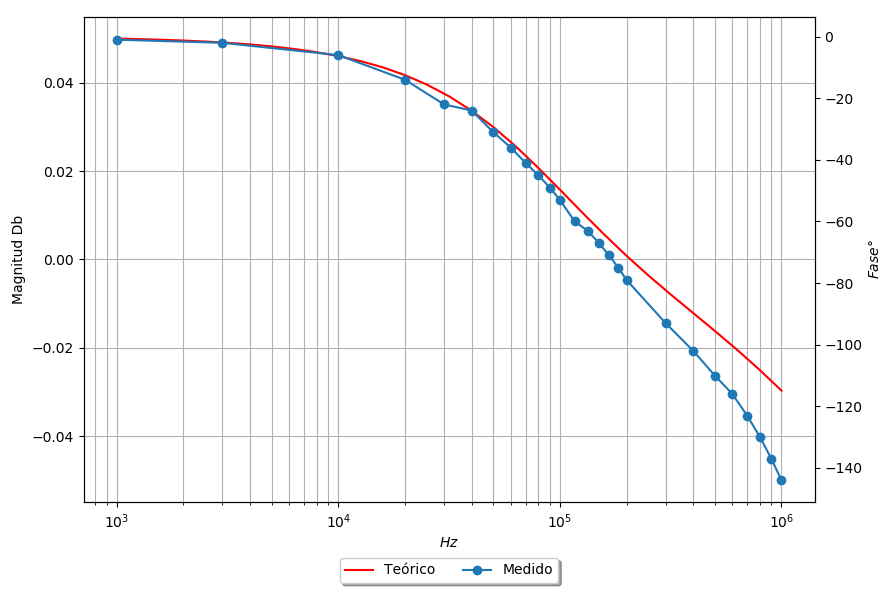
\includegraphics[width=0.8\textwidth, trim = {2.2cm 0 0 0},clip]{Ejercicio1/Imagenes/BodephC1_noinv.png}
	\caption{Diagrama de Bode en fase Caso 1.}
	\label{fig:BodephC1_noinv}
\end{figure} 

\begin{figure}[H]	
	\centering
	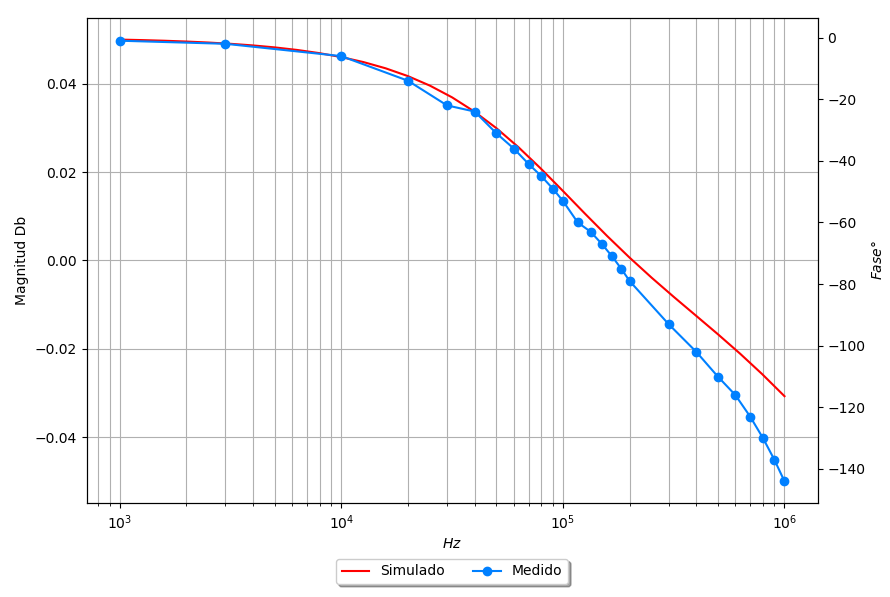
\includegraphics[width=0.8\textwidth, trim = {0 0 2cm 0},clip]{Ejercicio1/Imagenes/BodeC2_noinv.png}
	\caption{Diagrama de Bode en amplitud Caso 2.}
	\label{fig:BodeC2_noinv}
\end{figure} 
\begin{figure}[H]	
	\centering
	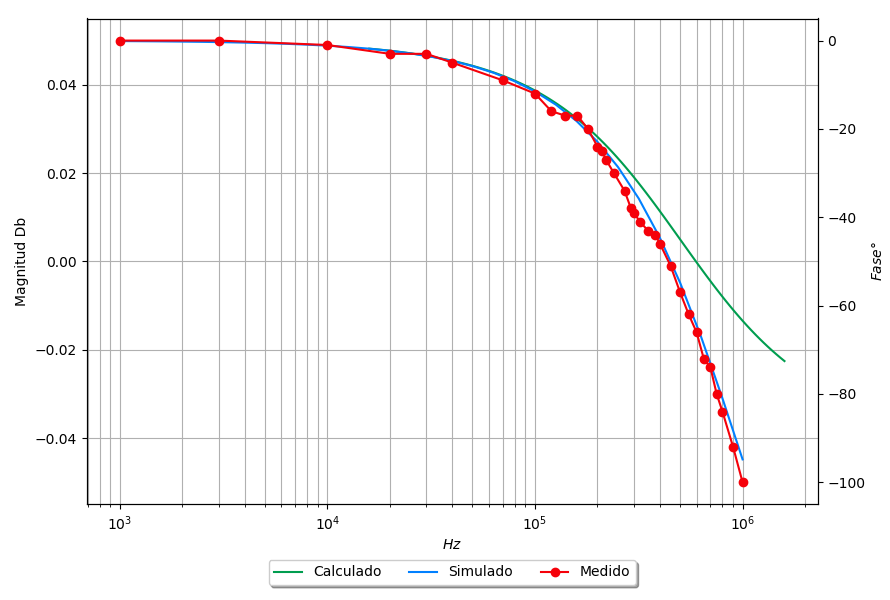
\includegraphics[width=0.8\textwidth, trim = {2.2cm 0 0 0},clip]{Ejercicio1/Imagenes/BodephC2_noinv.png}
	\caption{Diagrama de Bode en fase Caso 2.}
	\label{fig:BodephC2_noinv}
\end{figure} 

\begin{figure}[H]	
	\centering
	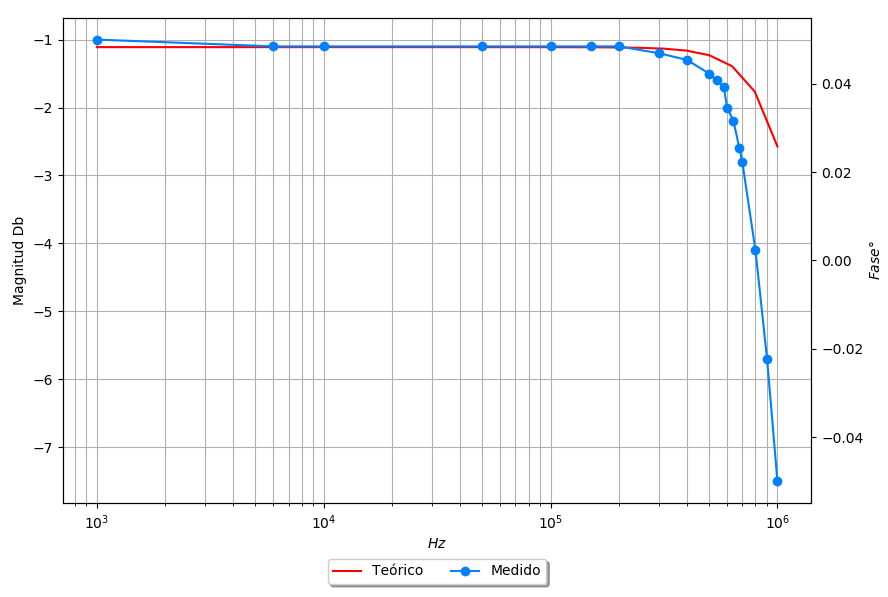
\includegraphics[width=0.8\textwidth, trim = {0 0 2cm 0},clip]{Ejercicio1/Imagenes/BodeC3_noinv.png}
	\caption{Diagrama de Bode en amplitud Caso 3.}
	\label{fig:BodeC3_noinv}
\end{figure} 
\begin{figure}[H]	
	\centering
	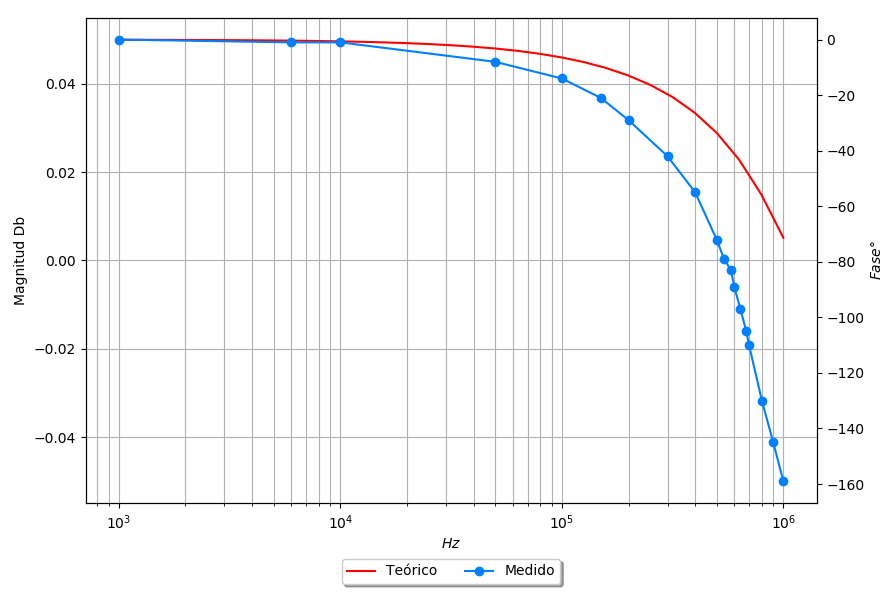
\includegraphics[width=0.8\textwidth, trim = {2.2cm 0 0 0},clip]{Ejercicio1/Imagenes/BodephC3_noinv.png}
	\caption{Diagrama de Bode en fase Caso 3.}
	\label{fig:BodephC3_noinv}
\end{figure} 

Se puede observar en todos los casos como la frecuencia de corte de las transferencias son próximas, mientras que las transferencias medidas y simuladas difieren de la teórica. Esto es más evidente al observar las discrepancias en (\ref{fig:BodephC1_noinv}), (\ref{fig:BodephC2_noinv}) y (\ref{fig:BodephC3_noinv}) a altas frecuencias. Esto se debe a las puntas del osciloscopio cuyas capacitancias son de aproximadamente $80 \ pF$. Al pasar a las altas frecuencias, este capacitor genera un filtro de segundo orden con el polo ya existente, atenuando la tensión de salida del circuito y generando en consecuencia que esta sea comparable con el ruido existente y dificultando las mediciones.

\subsubsection{Limitaciones.}
Algunas limitaciones con las cuales se lidiaron al utilizar este operacional fueron la intervención del Slew-Rate, el efecto de Cross-Over y la saturación del mismo.

En el caso de que se quiera trabajar con una señal cuadrada de $1 \ Vpp$, en un rango de frecuencias de $0.3 \ MHz \sim 2 \ MHz$, con un Duty Cycle entre 20\% y 80\%, no será posible, dado que se presentaran problemas de Slew-Rate. Por otro lado, se observarán problemas de Cross-Over cuando la media de la señal no supere los $0.7 \ V$.
Viendo que el operacional LM324 no funciona para dichas aplicaciones, se encontraron X amplificadores operacionales que pueden ser utilizados con una señal de las características mencionadas. Considerando que posean un valor medio de $0 \ V$ y un DT de 50\% los cuales son: TL084,

\begin{center}
\textcolor{red}{\textbf{BUSCAR OPERACIONALES.}}
\end{center}

\end{document}